\documentclass[final,3p,times,11pt]{elsarticle}
\usepackage[USenglish]{babel}
\usepackage{amsmath,amssymb,amsthm, mathrsfs}
\usepackage{mathtools}
\usepackage{graphicx}
\usepackage{stmaryrd}
\usepackage[dvipsnames]{xcolor}
\usepackage{cancel}
\usepackage{ulem}
\usepackage{tabularx}
\usepackage{comment}
%\usepackage{subcaption}
%\usepackage[show]{ed}
%\usepackage{showkeys}
%\usepackage{showlabels}
%\usepackage[notcite,notref]{showkeys}
%\usepackage{refcheck}
% \usepackage[ruled,vlined]{algorithm2e}
\usepackage[linesnumbered,ruled,vlined]{algorithm2e}
\definecolor{Myblue}{rgb}{.2 0.4 1}

\usepackage{hyperref}
\hypersetup{
    %bookmarks=true,         % show bookmarks bar?
    colorlinks = true,       % false: boxed links; true: colored links
    % linkcolor=green
     %linkcolor=red,          % color of internal links (change box color with linkbordercolor)
     %citecolor=green,        % color of links to bibliography
    %filecolor=magenta,      % color of file links
    %urlcolor=cyan           % color of external links
}
%\usepackage{wrapfig}
%% The lineno packages adds line numbers. Start line numbering with
%% \begin{linenumbers}, end it with \end{linenumbers}. Or switch it on
%% for the whole article with \linenumbers after \end{frontmatter}.
%\usepackage{lineno}


% ==============   Macros  ====================
\newcommand{\mynabla}{\widetilde{\nabla}} 
\newcommand{\jump}[1]{[\![#1]\!]}
\newcommand{\HEcolor}[1]{{\textcolor{blue}{#1}}}
\newcommand{\TSVcolor}[1]{{\textcolor{orange}{#1}}}
\newcommand{\JLcolor}[1]{{\textcolor{violet}{#1}}} %violet
\newcommand{\Grids}{\boldsymbol{\chi}}

\newtheorem{theorem}{Theorem}%[section]
\newtheorem{VariationalForm}[theorem]{Variational Formulation}
% =============================================

\journal{}
\makeatletter
\def\ps@pprintTitle{%
 \let\@oddhead\@empty
 \let\@evenhead\@empty
 \def\@oddfoot{}%
 \let\@evenfoot\@oddfoot}
\makeatother




\begin{document}
\begin{frontmatter}
\title{Multi-fidelity Monte Carlo for uncertainty quantification in the free boundary Grad-Shafranov equation}


\author[umdcs]{Matthias Heinkenschloss}
\ead{heinken@rice.edu}
\address[umdcs]{Department of Computational Applied Mathematics \& Operations Research, Rice University.}
\author[umdm]{Jiaxing Liang}
\ead{jl508@rice.edu}
\address[umdm]{Department of Computational Applied Mathematics \& Operations Research, Rice University.}
% \author[UA]{Tonatiuh S\'anchez-Vizuet}
% \ead{tonatiuh@arizona.edu}
% \address[UA]{Department of Mathematics, The University of Arizona.}
\begin{abstract}
We investigate the Grad-Shafranov free boundary problem in Tokamak fusion reactors under the influence of parameter uncertainties. Using both traditional Monte Carlo and multi-fidelity Monte Carlo sampling approaches, we quantify the impact of these uncertainties on model predictions, emphasizing the statistical characterization of solution variability across diverse parameter regimes. Our numerical results reveals that the multi-fidelity Monte Carlo estimator achieves statistical accuracy comparable to the Monte Carlo approach. However, the multi-fidelity method demonstrates superior computational efficiency, achieving a cost reduction by a factor of ..., while preserving fidelity in representing plasma boundary dynamics and geometric parameters. This work underscores the efficiency of multi-fidelity frameworks in addressing the computational demands of uncertainty quantification in complex fusion reactor models, offering a robust pathway for enhancing predictive capabilities in plasma physics. 
\end{abstract}

\begin{keyword}
Multi-fidelity Monte Carlo Finite-Element \sep Parametric expectation, \sep Sparse Grid Stochastic Collocation \sep Uncertainty Quantification \sep Free Boundary Grad-Shafranov Problem.
%
\MSC[2020] 
\end{keyword}
\end{frontmatter}

% ========================================
\section{Introduction}\label{sec:intro}
% ========================================
The pursuit of controlled nuclear fusion as a clean and virtually limitless energy source has spurred extensive research into the physics of magnetic confinement in fusion reactors. At the core of this effort lies the Grad–Shafranov free-boundary problem, which governs the equilibrium state of plasma in axially symmetric geometries, such as those found in Tokamaks. The governing equation encapsulates the intricate interplay between magnetic fields and plasma pressure, which determines critical confinement and stability properties essential for efficient plasma performance. However, the predictive accuracy of these models is significantly challenged by uncertainties arising from measurement limitations, model assumptions, and operational variabilities. Addressing these uncertainties effectively requires advanced computational frameworks capable of robust statistical analysis, enabling accurate predictions of the plasma equilibrium response under diverse scenarios and ensuring reliable assessments of reactor designs and operations.

The Monte Carlo (MC) method is widely used to quantify uncertainty and estimate statistical properties of input random variables. However, its application is computationally prohibitive due to its notoriously slow convergence rate, which requires a high-fidelity numerical approximation of the nonlinear partial differential equations for a large number of sample realizations.  To mitigate this challenge, low-fidelity models have been proposed as computationally efficient alternatives. For instance, in \cite{ElLiSa:2022}, a low-fidelity model constructed using stochastic collocation was used to facilitate Monte Carlo sampling. In \cite{ElLiSa:2023}, several low-fidelity models, based on coarse spatial grids, were developed as surrogate models for multilevel Monte Carlo (MLMC) sampling. Additionally, other work (e.g., \cite{}) has explored generating low-fidelity models using stochastic collocation on coarse grids and integrating them with MLMC sampling. While these approaches reduce computational costs, the use of simplified surrogates introduces the risk of compromising accuracy. The trade-off between efficiency and accuracy is therefore critical and warrants careful investigation to balance computational savings with the reliability of results.

In this paper, we consider a multi-fidelity Monte Carlo (MFMC) method that uses the control variate approach to exploit correlations between the computationally expensive high-fidelity model and a series of appropriately chosen low-fidelity models. This method aims to further enhance sampling efficiency while preserving accuracy. Our goal is to demonstrate that this multi-fidelity approach can significantly accelerate sampling process while maintaining statistical fidelity, offering a practical and robust solution to the challenges posed by uncertainty quantification in plasma equilibrium modeling.


The paper is structured as follows. Section \ref{sec:Grad-Shafranov} introduces the Grad-Shafranov free boundary problem.  Section \ref{sec:SC} provides an overview of the sparse grid stochastic collocation technique used to construct low-fidelity models. Section \ref{sec:MC} and Section \ref{sec:MFMC} explore the surrogate-based Monte Carlo Finite Element and multilevel Monte Carlo Finite Element methods. Finally, Section \ref{sec:Num-Exp} presents numerical experimental results that evaluate the efficiency and accuracy of these strategies.

% Finally, the paper concludes with Section \ref{sec:Conclusion}, summarizing the key findings and contributions. 
% An appendix is included, containing technical mathematical details and proofs relevant to the problem and methods discussed.


% ========================================
\section{The Grad-Shafranov free boundary problem with uncertainty}\label{sec:Grad-Shafranov}
% ========================================
In magnetic confinement fusion reactors, atoms with light nuclei such as deuterium and tritium are injected into a chamber and heated to high temperature, ionizing to form a hot plasma. To maintain the conditions required for nuclear fusion, magnetic fields generated by external coils are used to confine the plasma and isolate it from the reactor wall. The confinement is governed by a balance between hydrostatic pressure and magnetic pressure generated from the external coils and internal plasma current. The equilibrium state, coupled with Maxwell’s equations,  is mathematically described by the Grad–Shafranov equation \cite{GrRu:1958, LuSc:1957, Shafranov:1958}. In axially symmetric tokamaks configurations, the problem simplifies to a two-dimensional formulation in the meridional $r$-$z$ plane using cylindrical coordinates $(r, z, \varphi)$. The equation determines the poloidal flux function $u(r,z)$ from 
%
\begin{subequations}\label{eq:FreeBoundary}
\begin{equation}
 -\nabla\,\cdot\,\left(\frac{1}{\mu r}\nabla u\right) = \left\{ \begin{array}{ll}
r\frac{d}{d u} p(u) + \frac{1}{2\,\mu r} \frac{d}{d u} g^2(u) & \text{ in } \Omega_p(u) \\
I_k/S_k & \text{ in } \Omega_{C_k} \\
0 & \text{ elsewhere, } 
\end{array}\right.
\end{equation}
%
where $\nabla$ and $\nabla\cdot$ denote the Cartesian gradient and divergence operators in two dimensions; the magnetic permeability $\mu$ is a constant $\mu_0$ in vacuum but varies as  $\mu = \mu(|\nabla u|^2/r^2)$ within ferromagnetic materials; the regions $\Omega_p$ and $\Omega_{C_k}$ correspond to the plasma confinement zone and the meridian cross-sections of external coils, respectively, with the latter carrying currents $I_k$ over areas $S_k$; the source term in $\Omega_p$ represents the toroidal component of the plasma current density, which depends non-linearly on the poloidal flux through the hydrostatic pressure $p(u)$ and toroidal magnetic field $g(u)$. We adopt experimentally motivated formulations for  $p(u)$ and $g(u)$ proposed in \cite{LuBr:1982} as
%
\begin{equation}\label{eq:source}
\frac{d}{d u}p( u) = \frac{\beta}{r_0}\left(1-u_N^{\alpha_1}\right)^{\alpha_2},  \qquad \qquad
\frac{1}{2}\frac{d}{d u}g^2(u) = \mu_0r_0(1-\beta)\left(1-u_N^{\alpha_1}\right)^{\alpha_2},
\end{equation}
\end{subequations}
%
where $u_N \in [0,1]$ is the normalized flux, scaled by the difference between its values at the \textit{magnetic axis} and the plasma boundary; the parameter $r_0$ denotes the outer radius of the vacuum chamber, $\alpha_1$ and $\alpha_2$ dictate the sharpness of the current peaks near the magnetic axis, and $\beta$, the \textit{poloidal beta}, measures the ratio of \textit{plasma pressure} to \textit{magnetic pressure}. The plasma boundary $\Omega_p$, delineated by the last closed streamline,  is dependent on $u$ and unknown a priori, introducing a \textit{free boundary problem}. The nonlinear dependence of the poloidal flux, combined with the magnetic permeability and the nonlinearity of $p(u)$ and $g(u)$, significantly contributes to the mathematical complexity of the Grad-Shafranov equation.

Let $\Omega$ be a bounded, Lipschitz domain enclosing the confinement region $\Omega_p$, the external coils $\Omega_{c_i}$, and all other structural components of the reactor.
The solution space $Z$ for \eqref{eq:FreeBoundary}, as defined in \cite{Gr:1999}, is
%
\begin{equation}\label{eq:Soln_space}
    Z:=\left\{u:\Omega\rightarrow \mathbb{R} \,\Bigg| \,\int_\Omega u^2rdrdz<\infty; \,  \int_\Omega\frac{|\nabla u|^2}{r}drdz<\infty; \, u(0,z)=0 \right\}\cap C^0(\overline{\Omega}),
\end{equation}
%
ensuring finite energy and continuity over $\overline\Omega$. The corresponding inner product and energy norm are
%
\[
    \langle u,v\rangle_Z := \int_{\Omega} \frac{1}{r} \nabla u\cdot\nabla v \;\;drdz,\qquad \| u \|_{Z} :=\left(\int_\Omega\frac{|\nabla u|^2}{r} drdz\right)^{1/2}.
\]
%
In practice, the equilibrium state of the plasma is vulnerable to uncertainties arising from sources such as measurement inaccuracies and operational fluctuations. These uncertainties manifest themselves as stochastic variations in the solution and its derived quantities, influencing the stability and performance of plasma confinement. This paper investigates the impact of parametric uncertainties on two key factors: the current intensities $I_k$ of the external coils and the parameters governing the source term \eqref{eq:source}. To model these uncertainties, we define a $d$-dimensional random variable $\boldsymbol \omega :=(\omega_1,\ldots,\omega_d)$,  where each component $\omega_i$ is treated as an independent random variable characterized by a probability density function $\pi_k$. The baseline values for these parameters are denoted by the vector $\boldsymbol{\widetilde{\omega}} = (\widetilde{\omega}_1, \ldots, \widetilde{\omega}_d)$. Assuming a uniform distribution for each parameter, centered around its corresponding baseline value $\widetilde{\omega}_i$ and perturbed by a relative magnitude $\tau$, the joint probability density function $\pi(\boldsymbol{\widetilde{\omega}})$ and the associated $d$-dimensional parameter space $W$ are
%
\begin{equation}
\label{eq:ParameterSpace}
 \pi \left(\boldsymbol{\omega}\right)=\prod_{k=1}^{d} \pi_k\left(\omega_{k}\right)=\prod_{k=1}^{d} \frac{1}{2\tau |\widetilde{\omega}_k|}, \qquad  
    W := \prod_{k=1}^{d}\left[\widetilde{\omega}_k-\tau \left\vert \widetilde{\omega}_k\right\vert,\widetilde{\omega}_k+\tau \left\vert \widetilde{\omega}_k \right\vert\right].
\end{equation}
%
Incorporating stochasticity into the current intensities and the source function requires solving for a solution operator $u(\cdot, \boldsymbol{\omega}): W \to Z$, which maps the realizations of the random variable $\boldsymbol \omega$ to the corresponding solutions of the free-boundary problem \eqref{eq:FreeBoundary}. To address the variability introduced by stochastic parameters, we adopt the {\it weighted Bochner space} framework, which provides a rigorous way to quantify combined spatial and parametric variability. For a stochastic function $u: W\to Z$, we consider function space $L^2(W,Z)$, consisting of functions with finite second moments, defined as
%
\[
L^2(W,Z) = \{u:W\rightarrow Z\big\vert u \text{ is strongly mearurable and }\int_{W}\left\|u(\cdot,\boldsymbol{\omega})\right\|_{Z}^2\pi(\boldsymbol{\omega})d\boldsymbol{\omega}<+\infty\},
\]
%
and the associated norm is defined as
\[
\left\Vert u \right\Vert_{L^2(\boldsymbol W,Z)} =
    \left(\int_{\boldsymbol W} \left\Vert u(\cdot,\omega)  \right\Vert_{Z}^2 \pi(\boldsymbol{\omega})d\boldsymbol{\omega} \right)^{1/2} = \left(\mathbb{E}\left[\left\Vert u(\cdot,\omega)  \right\Vert_{Z}^2\right]\right)^{1/2}\,. 
\]

The goal of this paper is to explore the propagation of uncertainty and efficiently approximate the parametric expectation of $u(\cdot,\boldsymbol \omega)$
%
 \begin{equation}
 \label{eq:QoI}
      \mathbb{E}\left(u(\cdot,\boldsymbol \omega)\right)=\int_W u(\cdot,\boldsymbol{\omega})\pi(\boldsymbol\omega)d\boldsymbol{\omega},
 \end{equation}
%
and to compute some derived quantities from \eqref{eq:QoI}, such as the plasma boundary and features of solutions such as the locations of x-points. 


To achieve computational efficiency, we use sampling techniques including Monte Carlo and multi-fidelity Monte Carlo methods. The high-fidelity model in the multi-fidelity Monte Carlo framework is implemented using the finite element-based solver {\tt FEEQS.m} \cite{Heumann:feeqsm} -- a lightweight Matlab implementation of the {\tt CEDRES++} code \cite{FaHe:2017,CEDRES}, developed by Holger Heumann and collaborators; it implements a piecewise linear Finite Element discretization of a weak formulation of \eqref{eq:FreeBoundary} and incorporates a globalized variant of Newton's method to resolve its inherent nonlinearity. Hereafter, we refer to this solver as the  {\it direct solver}. Moreover, the multi-fidelity framework relies on a sequence of low-fidelity models to mitigate the computational cost associated with the high-fidelity model. To construct these low-fidelity models for $u(\cdot, \boldsymbol{\omega})$, we use the sparse grid stochastic collocation method \cite{BaNoRi:2000, KlBa:2005, MaNi:2009, Sm:1963}.






% Incorporating the uncertainty and 
% %
% \begin{equation}\label{eq:FreeBoundarya}
%  -\nabla\,\cdot\,\left(\frac{1}{\mu(u(\cdot, \boldsymbol{\omega})) r}\nabla u(\cdot, \boldsymbol{\omega})\right) = \left\{ \begin{array}{ll}
% \frac{d}{du} p(u(\cdot, \boldsymbol{\omega})) + \frac{1}{2\,\mu r} \frac{d}{du} g^2(u(\cdot, \boldsymbol{\omega})) & \text{ in } \Omega_p(u(\cdot, \boldsymbol{\omega})) \\
% I_k(\boldsymbol\omega)/S_k & \text{ in } \Omega_{C_k} \\
% 0 & \text{ elsewhere, } 
% \end{array}\right.
% \end{equation}






% ============================================================
\section{Sparse grid stochastic collocation}\label{sec:SC}
% ============================================================
This section provides a brief overview of the sparse grid stochastic collocation approach \cite{BaNoRi:2000, KlBa:2005, MaNi:2009, Sm:1963}, demonstrated using a generic solution $u$. 

The method starts by defining a univariate set of $m_i$ collocation nodes $X^i = \left\{x_1^i,\ldots, x_{m_i}^i\right\}$ over the interval $[-1,1]$. Using these nodes, a univariate interpolation operator is built as $I_{X^{i}}[u]:=\sum_{j=1}^{m_{i}} u(\cdot, x_j^i)\phi_j$, where the basis function $\phi_k(x_j^i)$ is the Kronecker delta, evaluating to 1 when $k=j$ and $0$ otherwise. To extend this approach to high-dimensional parameter space, the method combines univariate nodes across multiple dimensions using a tensor product. Instead of using a full tensor grid -- which grows exponentially with the number of dimensions $d$ -- the sparse grid framework selects fewer nodes $m_i$ per dimension, drastically reducing computational costs while maintaining accuracy. The {\it sparse grid nodes} for a domain of dimension $d$ and {\it level} $q\; (\text{where }q\ge d)$ are defined as
%
\begin{equation*}
H(q,d) = \bigcup_{q-d+1\le|\boldsymbol{i}|\le q} \left(X^{i_1}\times \cdots\times X^{i_d}\right)\in [-1,1]^d, 
\end{equation*}
where $|\boldsymbol{i}| = i_1+\ldots+i_d$ specifies the refinement rule. These nodes form a sparse representation of the domain, capturing the essential features of $u$ with fewer evaluations than a full grid. 


For our problem, the collocation nodes are selected as the extrema of the Chebyshev polynomials \cite{BaNoRi:2000, ClCu:1960}, with the $j$-th node calculated as $x_j^i=-\cos (\pi(j-1)/(m_i-1))$ for $j=1, \ldots, m_i$. The number of nodes is determined so that $m_1 =1$ and $m_i = 2^{i-1}+1$ for $i\ge 2$. This specific choice ensures that the univariate nodal sets $X^i$ exhibit a {\it nested} structure, satisfying $X^i\subset X^{i+1}$. Consequently, the multidimensional sparse grid nodes inherit this nesting property,  resulting in
%
\begin{equation}
\label{eq:NestedColPts}
H(q,d)\subset H(q+1,d),\quad \text{and}\quad H(q,d) = \bigcup_{|\boldsymbol{i}|=q} \left(X^{i_1}\times \cdots\times X^{i_d}\right).
\end{equation}
%
This hierarchical nesting allows for the reuse of function evaluations at coarser levels when constructing finer levels, further enhancing computational efficiency compared to non-nested grids. Interpolation over the hierarchical sparse grid nodes $H(q,d)$ is performed using the {\it Smolyak quadrature formula}, which combines univariate interpolation operators across dimensions as
%
\begin{equation}
\label{eq: Smolyak_Quad_formula}
\mathcal{S}_{q, d}[u] = \sum_{q+1\le |\boldsymbol{i}|\le q+d} (-1)^{q+d-|\boldsymbol{i}|} \binom{d-1}{q+d-|\boldsymbol{i}|}\cdot \left(\mathrm I_{X^{i_1}}\otimes\cdots\otimes \mathrm I_{X^{i_d}}\right) [u].
\end{equation} 
%
This method efficiently computes high-dimensional interpolations by exploiting the sparsity and hierarchical structure of the grid, providing an effectively balances between computational efficiency and precision, making it particularly suited for solving deterministic parametrized problems involving high-dimensional uncertainties.



% Let $N$ denote the number of sparse grid nodes. The sparse grid stochastic collocation method is equivalent to solving $N$ deterministic parametrized problems \eqref{eq:FreeBoundary} at each nodal point in $H(q,d)$.

% For our model problem, the sparse grid stochastic collocation method constructs the surrogate function $ \mathcal{S}_{q,d}(u)$ as per \eqref{eq: Smolyak_Quad_formula} by computing the direct solution of the discrete version of \eqref{eq:FreeBoundary} at isotropic sparse grid nodes \eqref{eq:NestedColPts} with the Clenshaw-Curtis quadrature abscissa  \cite{BaNoRi:2000,ClCu:1960}. 

As discussed in \cite{NoTeWe:2008,TeJaWe:2015}, consider the function $u \in C^0(W,Z)$, where the parameter space $W$ and the solution space $Z$ are defined in \eqref{eq:ParameterSpace} and \eqref{eq:Soln_space} respectively. Let the interval in the $k$-th dimension be defined as $W_k = \left[\widetilde{\omega}_k-\tau \left\vert \widetilde{\omega}_k\right\vert, \widetilde{\omega}_k+\tau \left\vert \widetilde{\omega}_k\right\vert\right]$. The complementary multi-dimensional parameter space that excludes the $k$-th dimension is 
%
\[
W_k^c = \prod_{i=1, i\neq k}^d W_i.
\]
%
Now, for any fixed element $\omega_k^c \in W_k^c$, and for each $\omega_k\in W_k$, we assume the function $u(\cdot,\omega_k,\omega_k^c): W_k \rightarrow C^0(W_k^c;Z)$ admits an analytic extension  $u(\cdot, z,\omega_k^c)$ in the complex plane, specifically in the region 
%
\[
W_k^{*}:=\{z\in \mathbb{C}: \text{dist} (z,W_k)\le \iota_k \;\text{ for some } \iota_k>0\},
\]
%
where $\iota_k$ denotes the proximity of the analytic extension to the real interval $W_k$. Under these assumptions, the interpolation error associated with the sparse grid method demonstrates an algebraic convergence rate
%
\begin{equation} \label{eq:coll-error-bound_2}
  \big\|u-\mathcal{S}_{q, d} (u)\big\|_\infty = C P^{-\mu},
\end{equation}
%
where $P$ denotes the sparse grid node count, $C$ is a constant dependent on dimension $d$ and analytic extension proximity to the interval $W_k$, and $\displaystyle \mu$ is related to the dimension of parameter space and function's analytic extension in the complex plane.

% Compared to the regularity assumption of $u$ in \cite{ElLiSa:2022}, the assumption for \eqref{eq:coll-error-bound_2} is stronger in the sense that the solution $u$ with respect to the random variable $\boldsymbol{\omega}$ can be analytically extended into the complex plane region by varying with one dimension of the random variable while keeping the other dimensions fixed.  This enhancement allows for a tighter interpolation error bound compared to the regularity assumption in \cite{ElLiSa:2022}.



% ====================================================
\section{Monte Carlo estimator}\label{sec:MC}
% ====================================================
To estimate the expectation in \eqref{eq:QoI}, Monte Carlo sampling is typically used.  Let $u_h (\cdot, \boldsymbol{\omega})$ denote a discrete approximation of $u(\cdot, \boldsymbol{\omega})$ for the stochastic version of \eqref{eq:FreeBoundary}, obtained using a spatial discretization characterized by the mesh parameter $h$ and consisting of $M$ nodes. For simplicity, we write $u$ and $u_h$ as $u(\cdot,\boldsymbol \omega)$ and $u_h(\cdot,\boldsymbol \omega)$ respectively. The Monte Carlo Finite-Element estimator $A^{\text{MC}}_{N}$ is defined as the sample mean of $N$ independent and identically distributed (i.i.d.) realizations $\boldsymbol{\omega}^{(1)},\ldots,\boldsymbol{\omega}^{(N)}$
%
\begin{equation}\label{eq:MC_estimator}
    A^{\text{MC}}_{N} := \frac{1}{N}\sum_{i=1}^{N} u_{h}(\cdot, \boldsymbol{\omega}^{(i)}),
\end{equation}
%
where $\mathbb{E}(A^{\text{MC}}_{N}) = \mathbb{E}(u_{h})$, $\mathbb{V}(A^{\text{MC}}_{N}) = \mathbb{V}( u_{h})/{N}$ and $\mathbb{V}(u) := \mathbb{E}\left(\left\Vert u - \mathbb{E}(u)\right\Vert_Z^2\right)$. The central limit theorem ensures that as $N$ approaches infinity, the estimator \eqref{eq:MC_estimator} converges in distribution to $\mathbb{E}(u)$. While this guarantees asymptotic behavior, the normalized \textit{mean squared error} (nMSE) offers a quantitative measure of how much the estimator deviates from the true value in the mean-square sense. Normalized by $\left\Vert\mathbb{E}(u) \right\Vert_{Z}^2$, the nMSE is defined as
%
 \[
\mathcal{E}_{A^{\text{MC}}_{N}}^2:=\frac{\mathbb E\left[\left\Vert\mathbb{E}(u)-A^{\text{MC}}_{N} \right\Vert_{Z}^2\right]}{\left\Vert\mathbb{E}(u) \right\Vert_{Z}^2}.
\] 
%
The nMSE for the Monte Carlo estimator can be decomposed into two components: a bias term, reflecting the discretization of $u$ using $u_h$, and the statistical error, arising from finite sampling. The decomposition is expressed as
%
\[
\mathcal{E}_{A^{\text{MC}}_{N}}^2 = \frac{\left\Vert\mathbb{E}(u)-\mathbb{E}(u_{h}) \right\Vert_{Z}^2+\mathbb E\left[\left\Vert \mathbb{E}(u_{h}) -A^{\text{MC}}_{N} \right\Vert_{Z}^2\right]}{\left\Vert\mathbb{E}(u) \right\Vert_{Z}^2} = \frac{\left\Vert\mathbb{E}(u)-\mathbb{E}(u_{h}) \right\Vert_{Z}^2}{\left\Vert\mathbb{E}(u) \right\Vert_{Z}^2}+\frac{\mathbb{V}\left( u_{h}\right)}{N\left\Vert\mathbb{E}(u) \right\Vert_{Z}^2}=\mathcal{E}_{\text{Bias}}^2 + \mathcal{E}_{\text{Stat}}^2.
\]
%
For the bias error, we assume that the sample-wise discretization error satisfies
%
\begin{equation*} \label{eq:Assumption_uhA}
\|u(\cdot, \boldsymbol\omega^{(i)})-u_h(\cdot,\boldsymbol\omega^{(i)})\|_Z\leq C_m(\boldsymbol\omega^{(i)})M^{-\alpha}\,,
\end{equation*}
%
where $C_m(\boldsymbol\omega^{(i)})$ is a constant depending only on the geometry of the spatial domain and the particular realization $\boldsymbol\omega^{(i)}$, $\alpha>0$ is the convergence rate of spatial discretization, and \JLcolor{$M$ is the number of spatial grid nodes.} Given a user-specified threshold $\epsilon^2$  for the nMSE, we introduce a {\it splitting ratio} $\theta \in (0,1)$, which allocates the total error budget $\epsilon^2$ between bias and statistical components requiring that
%
\begin{equation} \label{eq:error-budget}
%\textcolor{red}{\|u-u_h\|_{L^2(\boldsymbol W,Z)}\le C_mM^{-\alpha}\le \theta_1\epsilon},\qquad\text{ and }\qquad \|u_h-\widehat u_{h}\|_{L^2(\boldsymbol W,Z)} \le C_{p} P^{-\nu}\le \theta_2\epsilon\,.  
\mathcal{E}_{\text{Bias}}^2=\|u-u_h\|_{L^2(\boldsymbol W,Z)}\le C_mM^{-\alpha}= \theta\epsilon^2, \quad\quad \mathcal{E}_{\text{Stat}}^2 = \frac{\sigma_1^2}{N\left\Vert\mathbb{E}(u) \right\Vert_{Z}^2}=(1-\theta)\epsilon^2,
\end{equation}
where $C_m$ is independent of the sample and $\sigma_1^2 = \mathbb{V}\left( u_{h}\right)$. To satisfy the error constraints,  the required number of spatial nodes $M$ and sample size $N$ must satisfy
%
\begin{equation}
\label{eq:SLSGC_SL_SpatialGridsNo_n_SparseGridsNo}
M\ge \left(\frac{\theta\epsilon^2}{C_m}\right)^{-\frac 1 {\alpha}},\quad\quad  N \ge  \frac{\sigma_1^2}{\epsilon^2(1-\theta)\left\Vert\mathbb{E}(u) \right\Vert_{Z}^2},
\end{equation}
%
Since $M$ and $N$ are integers, we round them up to the smallest integers that satisfy \eqref{eq:SLSGC_SL_SpatialGridsNo_n_SparseGridsNo}. Assume the average cost of evaluating $u_{h}$ for a single sample is $C$. The total computational cost of estimating $\mathbb{E}\left(u_h\right)$ with $N$ samples is
%
\[
\mathcal{W}_\text{MC}  = CN=\frac{C\sigma_1^2}{\epsilon^2(1-\theta)\left\Vert\mathbb{E}(u) \right\Vert_{Z}^2}.
\]
%

% ====================================================
\section{Multi-fidelity Monte Carlo}\label{sec:MFMC}
% ====================================================
% examine two main sampling methods: Monte Carlo Finite-Element (MC-FE) and multifidelity Monte Carlo Finite-Element sampling methods (MFMC-FE).

% Let $u_h$ be a finite element discretized solution to \eqref{eq:FreeBoundary} as our high fidelity model. 
The Monte Carlo finite element estimator is often computationally expensive due to the extensive sampling on a fixed finite element discretization. This can become prohibitively costly, particularly under stringent accuracy requirements. To mitigate this challenge, we turn to multi-fidelity Monte Carlo sampling \cite{PeWiGu:2016}, an approach that combines high-fidelity models -- characterized by their accurate approximation of system behavior -- and low-fidelity models, which are computationally efficient albeit less detailed. The core of this approach is rooted in the {\it control variate} technique, which reduces the variance of the estimator by exploiting the statistical correlations between high- and low-fidelity models. By optimally allocating computational effort across these models, the multi-fidelity framework significantly decreases the reliance on expensive high-fidelity evaluations, ultimately lowering computational costs. Importantly, this strategy preserves the accuracy and robustness of the resulting estimator, offering a practical and efficient alternative to traditional high-fidelity-only Monte Carlo sampling. Below, we provide a brief overview of this method.

To approximate \eqref{eq:QoI}, the multi-fidelity Monte Carlo combines the high-fidelity model $u_{h,1}$ with a sequence of progressively less detailed but computationally cheaper low-fidelity models $u_{h,k}: W \rightarrow Z$ for $k=2,\ldots,K$. The fidelity of the models decreases as $k$ increases, with $u_{h,1}$ being the most accurate. For each model $u_{h,k}$, we define the variance and Pearson correlation coefficient between two models $u_{h,k}$ and $u_{h,j}$ as
%
\begin{equation*}
    \sigma_k^2 = \mathbb{V}\left(u_{h,k}\right),\qquad \rho_{k,j} = \frac{\text{Cov}\left(u_{h,k},u_{h,j}\right)}{\sigma_k\sigma_j}, \quad k,j=1,\dots, K,
\end{equation*}
%
where $\text{Cov}(u_{h,k},u_{h,j}) := \mathbb{E}[\langle u_{h,k} - \mathbb{E}(u_{h,k}), u_{h,j} - \mathbb{E}(u_{h,j})\rangle_Z]$ and $\rho_{k,k}=1$.
% The Multilevel Monte Carlo estimator is defined as
% \begin{equation}\label{eq:MLMC_estimator}
%     A^{\text{ML}} := A^{\text{MC}}_{L,N_L} + \sum_{k=2}^K \left(A^{\text{MC}}_{k-1,N_{k-1}} - A^{\text{MC}}_{k,N_{k-1}} \right),
% \end{equation}
The multi-fidelity Monte Carlo Finite-Element estimator $A^{\text{MF}}$ incorporates weighted corrections derived from low-fidelity models into the  Monte Carlo estimator of the high-fidelity model, defined as
%
\begin{equation}\label{eq:MFMC_estimator}
    A^{\text{MF}} := A^{\text{MC}}_{1,N_1} + \sum_{k=2}^K \alpha_k\left(\overline{A}_{k,N_k} - \overline{A}_{k,N_{k-1}} \right),
\end{equation}
%
where $A^{\text{MC}}_{1,N_1} $ is the Monte Carlo estimator for the high-fidelity model using $N_1$ samples, $\alpha_k$ are the weights for the correction terms, and $\overline{A}_{k,N_k}$ denotes the sample average of the $k$-th model based on $N_k$ samples. The sample average term $\overline{A}_{k,N_{k-1}}$ in each correction reuses the first $N_{k}$ samples from $\overline{A}_{k,N_{k}}$, requiring the condition $N_{k-1}\le N_k$ for $k=2,\ldots, K$. By partitioning the $N_k$ samples into two disjoint sets, one of size $N_{k-1}$ and the other of size $N_k - N_{k-1}$, we can reformulate the MFMC estimator \eqref{eq:MFMC_estimator} as
%
\begin{equation}\label{eq:MFMC_estimator_independent}
    A^{\text{MF}} = A^{\text{MC}}_{1,N_1} +  \sum_{k=2}^K \alpha_k\left(\frac{N_{k-1}}{N_{k}}-1\right)\left(A_{k,N_{k-1}}^{\text{MC}}- A_{k,N_k\backslash N_{k-1}}^{\text{MC}}\right),
\end{equation}
%
The weights in the correction terms of this reformulation  are now functions of the sample ratio between successive fidelity levels. This reformulation is crucial because it ensures that the samples used in  the two components $A_{k,N_{k-1}}^{\text{MC}}$ and $A_{k,N_k\backslash N_{k-1}}^{\text{MC}}$ of the low-fidelity corrections are independent. The MFMC estimator can be compactly written as
%
\[
A^{\text{MF}} = Y_1 + \sum_{k=2}^K \alpha_k Y_k,
\]
%
where $Y_k$ are defined as
%
\[
Y_1 :=A^{\text{MC}}_{1,N_1},\quad Y_k:=\left(\frac{N_{k-1}}{N_{k}}-1\right)\left(A_{k,N_{k-1}}^{\text{MC}}- A_{k,N_k\backslash N_{k-1}}^{\text{MC}}\right), k=2\ldots, K.
\]
%
It can be shown that $\mathbb{E}(Y_k) = 0$ for $k\ge 2$, which implies $\mathbb{E}(A^{\text{MF}}) = \mathbb{E}(u_{h,1})$, ensuring the unbiasedness of the estimator. Since the samples in two disjoint components of $Y_k$ are independent, the variances of $Y_k$ can be computed as
%
\[
\mathbb{V}\left(Y_1\right) = \frac{\sigma_1^2}{N_1}, \quad \mathbb{V}\left(Y_k\right) = \left(\frac{N_{k-1}}{N_{k}}-1\right)^2\left(\frac{\sigma_k^2}{N_{k-1}}+\frac{\sigma_k^2}{N_k-N_{k-1}}\right) = \left(\frac{1}{N_{k-1}} - \frac{1}{N_k}\right)\sigma_k^2.
\]
%
While $Y_k$ and $Y_j$ for $k\neq j, k,j=2,\cdots, K$ are dependent due to overlapping sample sets, it can be shown that $Y_k$ and $Y_j$ are uncorrelated. However, $Y_k$  is correlated with $Y_1$ since the samples used in $Y_k$ reuse those of $Y_1$. Using the covariance relation from \cite[Lemma~3.2]{PeWiGu:2016}, we express the covariance between $Y_1$ and $Y_k$ as
\[
\text{Cov}(Y_1,Y_k) = - \left(\frac{1}{N_{k-1}} - \frac{1}{N_k}\right)\rho_{1,k}\sigma_1\sigma_k.
\]
The variance of the multi-fidelity Monte Carlo estimator is
\begin{align}
    \nonumber
    \mathbb{V}\left(A^{\text{MF}}\right) &= \mathbb{V}\left(Y_1\right) + \mathbb{V}\left(\sum_{k=2}^K \alpha_kY_k\right)+2\;\text{Cov}\left(Y_1,\sum_{k=2}^K \alpha_k Y_k \right),\\
    \nonumber
    &=\mathbb{V}\left(Y_1\right) + \sum_{k=2}^K \alpha_k^2 \mathbb{V}\left(Y_k\right)+2\sum_{2\le k<j\le K} \alpha_k\alpha_j\; \text{Cov}(Y_k,Y_j) +2\sum_{k=2}^K \alpha_k\;\text{Cov}\left(Y_1, Y_k\right),\\
    % \nonumber
    % &=\mathbb{V}\left(Y_1\right) + \sum_{k=2}^K \alpha_k^2 \mathbb{V}\left(Y_k\right) +2\sum_{k=2}^K \alpha_k\;\text{Cov}\left(Y_1, Y_k\right),\\
    \label{eq:MFMC_variance}
    &=\frac{\sigma_1^2}{N_1} + \sum_{k=2}^K \left(\frac{1}{N_{k-1}} - \frac{1}{N_k}\right)\left(\alpha_k^2\sigma_k^2 - 2\alpha_k\rho_{1,k}\sigma_1\sigma_k\right).
\end{align}
%
Using the variance of the MFMC estimator, the nMSE for the multi-fidelity Monte Carlo estimator can be split as bias and statistical errors as
%
\[
\mathcal{E}_{A^{\text{MF}}}^2= \frac{\left\Vert\mathbb{E}(u)-\mathbb{E}(A^{\text{MF}}) \right\Vert_{Z}^2+\mathbb E\left[\left\Vert\mathbb{E}(A^{\text{MF}})-A^{\text{MF}} \right\Vert_{Z}^2\right]}{\left\Vert\mathbb{E}(u) \right\Vert_{Z}^2} =\frac{\left\Vert\mathbb{E}(u)-\mathbb{E}(A^{\text{MF}}) \right\Vert_{Z}^2}{\left\Vert\mathbb{E}(u) \right\Vert_{Z}^2}+ \frac{\mathbb{V}\left(A^{\text{MF}}\right)}{\left\Vert\mathbb{E}(u) \right\Vert_{Z}^2}=\mathcal{E}_{\text{Bias}}^2 + \mathcal{E}_{\text{Stat}}^2,
\]
%
\JLcolor{To ensure that the discretization error falls below $\theta\epsilon$, we estimate the number of spatial grid points $M_L$ required and the required spatial grid level $L$ as }
%
\begin{equation}
    \label{eq:SLSGC_MLS_SpatialGridsNo}
    M_L = M_0s^{-L} \ge \left(\frac{\theta\epsilon}{C_m}\right)^{-\frac 1 {\alpha}} \qquad \text{ and } \qquad     L = \left\lceil \frac{1}{\alpha}\log_s \left(\frac{c_m M_0^\alpha}{\theta\epsilon}\right) \right\rceil.
\end{equation}
%
Let $C_k$ denote the cost of generating a single sample from the $k$-th low-fidelity model, and $N_k$ represent the number of samples taken from that model. The total computational cost for the MFMC estimator is 
%
\[
\mathcal{W}^{\text{MF}} = \sum_{k=1}^K C_kN_k.
\]
%
Using the same splitting ratio $\theta$ between bias and statistical errors as introduced in the discussion of the Monte Carlo Finite-Element approach, our next goal is to identify the optimal sample sizes $N_k$ and weights $\alpha_k$ for the MFMC estimator \eqref{eq:MFMC_estimator_independent}. Towards this goal, we formulate an optimization problem such that the total sampling cost,
$\mathcal{W}^{\text{MF}}$, is minimized while ensuring that the normalized statistical error of the MFMC estimator  is controlled to achieve the required accuracy  $\mathcal{E}_{\text{Stat}}^2= (1-\theta)\epsilon^2$. Moreover, the optimization must enforce hierarchical ordering of the sample sizes, $N_{k-1}\le N_k$ for $k=2,\ldots, K$, and non-negativity of all sample sizes. This leads to the constrained optimization problem
%
\begin{equation}\label{eq:Optimization_pb_sample_size}
    \begin{array}{ll}
    \min \limits_{\begin{array}{c}\scriptstyle N_1,\ldots, N_K\in \mathbb{R} \\[-4pt]
\scriptstyle \alpha_2,\ldots,\alpha_K\in \mathbb{R}
\end{array}} &\displaystyle\sum\limits_{k=1}^K C_kN_k,\\
       \;\,\text{subject to} &\mathbb{V}\left(A^{\text{MF}}\right)- \left\Vert\mathbb{E}(u) \right\Vert_{Z}^2(1-\theta)\epsilon^2 = 0,\\[2pt]
        &\displaystyle -N_1\le 0, \\[1pt]
        &\displaystyle N_{k-1}-N_k\le 0, \quad\quad\, k=2\ldots,K.\\
    \end{array}
\end{equation}
%
The solution to \eqref{eq:Optimization_pb_sample_size}, which provides the real-valued optimal sample sizes and weights, is explicit presented in Theorem \ref{thm:Sample_size_est}. 
%
\begin{theorem}
\label{thm:Sample_size_est}
Consider a set of $K$ models, $u_k$ for $k=1,\ldots,K$, where each model is characterized by the standard deviation of its output $\sigma_k$, the correlation coefficient $\rho_{1,k}$ between the highest-fidelity model $u_{h,1}$ and the $k$-th low-fidelity model, and the computational cost per sample $C_k$. Assume the following conditions are satisfied
%
\begin{alignat*}{8}
    &(i)\;\; |\rho_{1,1}|>\ldots>|\rho_{1,K}|,& \qquad \qquad
    &(ii)\;\; \frac{C_{k-1}}{C_k}>\frac{\rho_{1,k-1}^2-\rho_{1,k}^2}{\rho_{1,k}^2-\rho_{1,k+1}^2},\;\;k=2,\ldots,K.
\end{alignat*}
%
Under these assumptions, the optimal weights $\alpha_k^*$ and sample sizes $N_k^*$, for $k=1,\ldots, K$ to the optimization problem \eqref{eq:Optimization_pb_sample_size} is
%
\begin{align}
    \label{eq:MFMC_coefficients}
    &\alpha_k^*=\frac{\rho_{1,k}\sigma_1}{\sigma_k},\\
    \label{eq:MFMC_SampleSize}
    &N_k^*=\frac{\sigma_1^2}{\left\Vert\mathbb{E}(u) \right\Vert_{Z}^2(1-\theta)\epsilon^2}\sqrt{\frac{\rho_{1,k}^2-\rho_{1,k+1}^2}{C_k}}\sum_{j=1}^K\sqrt{C_j\left(\rho_{1,j}^2-\rho_{1,j+1}^2\right)}, \quad \rho_{1,K+1}=0.
\end{align}
%
\end{theorem}
%

\begin{proof}
The optimization problem is approached with the method of Lagrange multipliers, where the auxiliary Lagrangian function $L$ incorporates multipliers $\lambda_0,\ldots, \lambda_K$ to enforce the constraints on the variance and sample sizes
%
\[
L = \sum_{k=1}^K C_kN_k +\lambda_0 \left(\frac{\sigma_1^2}{N_1} + \sum_{k=2}^K \left(\frac{1}{N_{k-1}} - \frac{1}{N_k}\right)\left(\alpha_k^2\sigma_k^2 - 2\alpha_k\rho_{1,k}\sigma_1\sigma_k\right)\right)-\lambda_1 N_1+\sum_{k=2}^K\lambda_k(N_{k-1} - N_k),
\]
%
To solve this, we apply the Karush-Kuhn-Tucker (KKT) conditions for \eqref{eq:Optimization_pb_sample_size}, leading to a system of equations for the partial derivatives of the Lagrangian with respect to the optimization variables $\alpha_k$ and $N_k$,  in addition to  primal feasibility, dual feasibility, and complementary slackness conditions
%
\begin{align*}
\frac{\partial L}{\partial \alpha_j}=0,\quad \frac{\partial L}{\partial N_k}&=0,\quad j=2\ldots,K, \quad k=1\ldots,K,\\
\mathbb{V}\left(A^{\text{MF}}\right)- \left\Vert\mathbb{E}(u) \right\Vert_{Z}^2(1-\theta)\epsilon^2 &= 0,\\
    N_{k-1}-N_k&\le 0, \quad k=2\ldots,K,\\
    -N_1&\le 0,\\[6pt]
    \lambda_1,\ldots,\lambda_K &\ge 0,\\
    \lambda_k(N_{k-1}-N_k)&=0,\quad k=2\ldots,K.\\
    \lambda_1 N_1&=0.
\end{align*}
%
The partial derivatives of the Lagrangian with respect to $\alpha_k$ and $N_k$ are computed as
%
\begin{align*}
    \frac{\partial L}{\partial \alpha_k}&=\lambda_0\left(\frac{1}{N_{k-1}} - \frac{1}{N_k}\right)\left(2\alpha_k\sigma_k^2 - 2\rho_{1,k}\sigma_1\sigma_k\right),\quad k=2,\dots,K,\\
    \frac{\partial L}{\partial N_1}&=C_1 + \lambda_0\left(-\frac{\sigma_1^2}{N_1^2} - \frac{\alpha_2^2\sigma_2^2-2\alpha2\rho_{1,2}\sigma_1\sigma_2}{N_1^2}\right)-\lambda_1+\lambda_2,\\
    \frac{\partial L}{\partial N_k}&=C_k+\lambda_0\left(\frac{\alpha_k^2\sigma_k^2 - 2\alpha_k\rho_{1,k}\sigma_1\sigma_k}{N_k^2}-\frac{\alpha_{k+1}^2\sigma_{k+1}^2 - 2\alpha_{k+1}\rho_{1,k+1}\sigma_1\sigma_{k+1}}{N_k^2}\right)-\lambda_k+\lambda_{k+1}, \quad k=2,\dots,K-1,\\
    \frac{\partial L}{\partial N_K}&=C_K + \lambda_0\left(\frac{\alpha_K^2\sigma_K^2 - 2\alpha_K\rho_{1,K}\sigma_1\sigma_K}{N_K^2}\right)-\lambda_K.
\end{align*}
%
By solving the equation $\partial L/\partial \alpha_k=0$, the optimal weights $\alpha_k^*$ are determined as
%
\[
\alpha_k^*=\frac{\rho_{1,k}\sigma_1}{\sigma_k}.
\]
%
Substituting $\alpha_k^*$ into $\partial L/\partial N_k=0$ yields a representation for $C_k$ in terms of the sample sizes $N_k$, variance contributions, correlation coefficients, and the Lagrangian multipliers
%
\begin{equation*}
    C_k=\frac{\lambda_0\sigma_1^2}{N_k^2}\left(\rho_{1,k}^2-\rho_{1,k+1}^2\right)+\lambda_k-\lambda_{k+1},\quad \text{for} \quad k=1,\ldots,K-1,\quad C_K=\frac{\lambda_0\sigma_1^2}{N_K^2}\rho_{1,K}^2+\lambda_K.
\end{equation*}
%
 As shown by  \cite{PeWiGu:2016}, the global minimizer is achieved when the inequality constraints are inactive ($\lambda_k$=0, $k=1,\dots, K$) in the complementary slackness conditions, indicating that the sample sizes strictly increase with $k$ ($N_{k-1}< N_k$ for $k=2,\ldots, K$). This results in the expression for the optimal sample sizes
% \[
% N_1 = \sigma_1\sqrt{\lambda_0}\sqrt{\frac{1-\rho_{1,2}^2}{C_1}}, \quad N_k = \sigma_1\sqrt{\lambda_0}\sqrt{\frac{\rho_{1,k}^2-\rho_{1,k+1}^2}{C_k}}, \quad N_K = \sigma_1\sqrt{\lambda_0}\sqrt{\frac{\rho_{1,K}^2}{C_K}},
% \]
% or we can simplify the notation as
\begin{equation}
\label{eq:sample_size_1}
    N_k = \sigma_1\sqrt{\lambda_0}\sqrt{\frac{\rho_{1,k}^2-\rho_{1,k+1}^2}{C_k}},\quad \text{with}\quad  \rho_{1,K+1}=0 \quad k=1,\ldots,K.
\end{equation}
% \frac{1}{N_k} = \frac{1}{\sigma_1\sqrt{\lambda_0}}\sqrt{\frac{C_k}{\rho_{1,k}^2-\rho_{1,k+1}^2}},
Using the optimal coefficients $\alpha_k^*$ and sample size estimations $N_k$ in \eqref{eq:sample_size_1}, the variance \eqref{eq:MFMC_variance} of the multi-fidelity Monte Carlo estimator becomes
%
\begin{equation*} \label{eq:MFMC_variance2}
    \mathbb{V}\left(A^{\text{MF}}\right) = \frac{\sigma_1}{\sqrt{\lambda_0}}\sum_{k=1}^K\sqrt{C_k\left(\rho_{1,k}^2-\rho_{1,k+1}^2\right)},\quad \text{with}\;\;\rho_{K+1}=0.
\end{equation*}
%
To satisfy the equality constraint for the variance,  we solve for $\sqrt{\lambda_0}$
%
\[
\sqrt{\lambda_0} = \frac{\sigma_1}{\left\Vert\mathbb{E}(u) \right\Vert_{Z}^2(1-\theta)\epsilon^2}\sum_{k=1}^K\sqrt{C_k\left(\rho_{1,k}^2-\rho_{1,k+1}^2\right)}.
\]
%
Substituting $\sqrt{\lambda_0}$ into  the equation for \eqref{eq:sample_size_1}, we obtain an estimate for the optimal sample sizes
%
\[
N_k^* = \frac{\sigma_1^2}{\left\Vert\mathbb{E}(u) \right\Vert_{Z}^2(1-\theta)\epsilon^2}\sqrt{\frac{\rho_{1,k}^2-\rho_{1,k+1}^2}{C_k}}\sum_{j=1}^K\sqrt{C_j\left(\rho_{1,j}^2-\rho_{1,j+1}^2\right)}.
\]
%
Note that by ensuring the condition $(ii)$ is satisfied, we can guarantee that $N_k$ increases strictly as $k$ grows. 
\end{proof}

The total sampling cost $\mathcal{W}^\text{MF}$ is derived from the sample size estimates
$N_k^*\in \mathbb{R}$ obtained in Theorem \ref{thm:Sample_size_est} as
%
\begin{equation}\label{eq:MFMC_sampling_cost}
    \mathcal{W}^\text{MF} = \sum_{k=1}^K C_k N_k^* = \frac{\sigma_1^2}{\left\Vert\mathbb{E}(u) \right\Vert_{Z}^2(1-\theta)\epsilon^2}\left(\sum_{k=1}^K\sqrt{C_k\left(\rho_{1,k}^2 - \rho_{1,k+1}^2\right)}\right)^2.
\end{equation}
%
However, since the correlation parameters and costs are unknown in practice, these quantities must be estimated based on sample data. Additionally, sample sizes should be rounded to the nearest integers for implementation. Thus, we use the ceiling function
$\left\lceil N_k \right\rceil$ to represent the sample size, which leads to the lower and upper bounds on the sampling cost
%
\begin{equation}\label{eq:sampling_cost_bound}
    \sum_{k=1}^K C_kN_k\le \sum_{k=1}^K C_k \left\lceil N_k\right\rceil<\sum_{k=1}^K C_kN_k + \sum_{k=1}^K C_k,
\end{equation}
%
where the term $\sum_{k=1}^K C_k$ results from the fact that $N_k\le \left\lceil N_k\right\rceil< N_k+1$. Let $B_k = C_k\left(\rho_{1,k}^2 - \rho_{1,k+1}^2\right), k=1,\dots, K$. In general, the behavior of $B_k$ depends on the product of $C_k$ and $\left(\rho_{1,k}^2 - \rho_{1,k+1}^2\right)$. $B_k$ can decay, grow and stay the same as $k$ increases. The total sampling cost \eqref{eq:MFMC_sampling_cost} can be rewritten as 
%
\begin{equation*}\label{eq:MFMC_sampling_cost_2}
    \mathcal{W}^{\text{MF}} = \sum_{k=1}^K C_k N_k = \frac{\sigma_1^2}{\left\Vert\mathbb{E}(u) \right\Vert_{Z}^2(1-\theta)\epsilon^2}\left(\sum_{k=1}^K\sqrt{B_k} \right)^2.
\end{equation*}
%
Then condition (ii) indicates that
\begin{equation}
    \frac{\sqrt{B_{k}}}{\sqrt{B_{k-1}}}>\frac{C_{k}}{C_{k-1}}, \quad k=2,\ldots,K.
\end{equation}
In the asymptotic regime when $K$ is large, the behavior of $\sqrt{B_k}$ can decay, grow, or stay the same. If $\sqrt{B_k}$ decays as $k$ increases, the decay of $\sqrt{B_k}$ is slower than the decay of $C_k$. This indicates that in all scenarios, as $k$ grows, we should expect the impact of $\sum_{k=1}^K C_k$  in \eqref{eq:sampling_cost_bound} is negligible  as $\sum_{k=1}^K C_kN_k$. As a result, the sampling cost using the integer sample size should behave like \eqref{eq:MFMC_sampling_cost}. Thus, using the optimal sample estimation $\left\lceil N_k\right\rceil$, we obtain the total sampling cost of multifidelity estimator (value of the objective function) as
\begin{equation}\label{eq:MFMC_sampling_cost_efficiency}
    \mathcal{W}^\text{MF} = \frac{\sigma_1^2}{\left\Vert\mathbb{E}(u) \right\Vert_{Z}^2(1-\theta)\epsilon^2}\left(\sum_{k=1}^K\sqrt{C_k\left(\rho_{1,k}^2 - \rho_{1,k+1}^2\right)}\right)^2.
\end{equation}

% Using the fact that $N_k$ increases and the value of $\alpha_k$, we observe that the MFMC estimator variance $\mathbb{V}\left(A^{\text{MFMC}}\right)$ in \eqref{eq:MFMC_variance2} always decreases as the model number $K$ increases. This reflects the fact that the low fidelity models are used as control variates to reduce the variance of the high fidelity model. However, this $K$ cannot be arbitrarily large, since the first summation term in \eqref{eq:MFMC_sampling_cost} grows, the second summation reflect the variance decay of the MFMC estimator. Thus this is a tie between these two terms. If $K$ is sufficiently large,  in order to achieve an optimal sampling cost, we need to study the decay and growth of these two terms. We will choose the $K$ such that the product of two summation terms in \eqref{eq:MFMC_sampling_cost} is minimum, i.e. If $K$ is sufficiently large, we need to find $K\in \mathbb{N}$ such that 
% \begin{equation}\label{eq:Optimal_K}
%    K = \text{argmin} \sum_{k=1}^K\sqrt{\left(\rho_{1,k}^2 - \rho_{1,k+1}^2\right)C_k}\sum_{k=1}^K\left(\sqrt{\frac{C_k}{\rho_{1,k}^2 - \rho_{1,k+1}^2}} - \sqrt{\frac{C_{k-1}}{\rho_{1,{k-1}}^2 - \rho_{1,k}^2}}\right)\rho_{1,k}^2. 
% \end{equation}


Our surrogate functions are built via a stochastic collocation approach with the same sparse grid nodes on a family of spatial meshes $\{\mathcal{T}_k\}$ of decreasing resolution, with a decreasing number of grid nodes $\{M_k,\}_{0\le k \le K}$ that, we will assume, satisfy
%
\begin{equation}
\label{eq:MeshGrowth}
M_k = s M_{k-1} \qquad \text{ for } s>1.
\end{equation}
%







\begin{theorem}
\label{thm:Sample_cost_est}
Let $u_{h,k}$ be $K$ models that satisfy the following conditions
Suppose there exist positive constants $\alpha, \beta, \gamma$ such that
%
\begin{alignat*}{8}
    &(i)\;\; |\rho_{1,1}|>\ldots>|\rho_{1,K}|,& \qquad \qquad
    &(ii)\;\; \frac{C_{k-1}}{C_k}>\frac{\rho_{1,k-1}^2-\rho_{1,k}^2}{\rho_{1,k}^2-\rho_{1,k+1}^2},\;\;k=2,\ldots,K, \quad \rho_{1,K+1}=0,\\
    &(iii)\;\; \left\Vert\mathbb{E}\left(u-u_{h,k}\right)\right\Vert_Z=\mathcal{O}\left( M_k^{-\alpha}\right),& \qquad \qquad
    &(iv)\;\; C_k=\mathcal{O}\left( M_k^{-\gamma}\right),\\
    &(v)\;\; \rho_{1,k-1}^2-\rho_{1,k}^2=\mathcal{O}\left( M_k^{\beta}\right).
\end{alignat*}
%
%
Then for $0<\epsilon$ there exist spatial grid level $K$ and sample size $N_\ell$ for which the multi-fidelity estimator $A^{\text{MF}}$ satisfies
\[
\left\Vert\mathbb{E}(u)-A^{\text{MF}} \right\Vert_{L^2(\boldsymbol W,Z)}<\epsilon\,\left\Vert\mathbb{E}(u) \right\Vert_{L^2( \boldsymbol W,Z)},
\]
with total sampling work bounded as
\begin{equation*}
    \mathcal{W}^{\text{MF}} \simeq 
%     \left\{\begin{array}{ll}
% \epsilon^{-2-\frac{\delta}{\nu}}, & \beta_1>1,\\
% \epsilon^{-2-\frac{\delta}{\nu}}\left\vert \log \epsilon \right\vert^2, & \beta_1 = 1,\\
% \epsilon^{-2-\frac{\delta}{\nu}-\frac{1 - \beta_1}{\alpha}}, & \beta_1<1.
% \end{array}
% \right.
\end{equation*}
\end{theorem}
\begin{proof}\label{eq:Sample_cost_est}

% Let 
% \[
% H_1:=\sum_{k=1}^L\sqrt{B_k},\quad H_2:=\sum_{j=1}^L\left(\frac{C_j}{\sqrt{B_j}} - \frac{C_{j-1}}{\sqrt{B_{j-1}}}\right)\rho_{1,j}^2,
% \]






% The cancellation of the two successive terms in the ratio representation on both sides of \eqref{eq:Theorem_cond_ii} indicates that 
% \[
% \frac{B_1}{C_1^2}C_k^2\le B_k\le \frac{B_K}{C_K^2}C_k^2, \quad k=1,\ldots,K.
% \]
% This indicates that
% \[
% \sqrt{\frac{1-\rho_{1,2}^2}{C_1}}\sum_{k=1}^K C_k\le \sum_{k=1}^K\sqrt{B_k}\le \sqrt{\frac{\rho_{1,K}^2}{C_K}}\sum_{k=1}^K C_k, \quad \text{or} \quad \sum_{k=1}^K
% \sqrt{B_k}\simeq \sum_{k=1}^K C_k,
% \]
% where $A\simeq B$ represents $a_1 B\le A\le a_2 B$ for positive $A$ and $B$, with constants $a_1, a_2$ independent of sample size $N_k$ but depends on model number $K$. This indicates that the sum in \eqref{eq:sampling_cost_bound} behaves in a similar style as $\sum_{k=1}^K C_k$. If $\epsilon$ is chosen sufficiently small, we can ignore the small term $\sum_{k=1}^K C_k$ in  \eqref{eq:sampling_cost_bound}. 





% Since $K$ is independent of $\epsilon$,  the total sampling cost behaves like $\epsilon^{-2}$. 

% Moreover, the inequality \eqref{eq:Theorem_cond_ii} also indicates that
% \[
% 0<\frac{C_L}{\sqrt{B_L}}\le \frac{C_k}{\sqrt{B_k}}<\frac{C_{k-1}}{\sqrt{B_{k-1}}}\le\frac{C_1}{\sqrt{B_1}},\quad k=2,\dots, L
% \]
% Therefore, the sequence $\frac{C_k}{\sqrt{B_k}} - \frac{C_{k-1}}{\sqrt{B_{k-1}}}\in (\frac{C_L}{\sqrt{B_L}} - \frac{C_{1}}{\sqrt{B_{1}}},0)$  is bounded. 

% Note that
% \[
% H_1:=\sum_{k=1}^L\sqrt{B_k}, \quad \sqrt{\frac{1-\rho_{1,2}^2}{C_1}}\sum_{k=1}^L C_k\le \sum_{k=1}^L\sqrt{B_k}\le \sqrt{\frac{\rho_{1,L}^2}{C_L}}\sum_{k=1}^L C_k, \quad H_1\uparrow \sqrt{\frac{\rho_{1,L}^2}{C_L}}\sum_{k=1}^L C_k \;\;\text{as}\;\; L\rightarrow \infty
% \]
% \[
% H_2:=\sum_{j=1}^L\left(\frac{C_j}{\sqrt{B_j}} - \frac{C_{j-1}}{\sqrt{B_{j-1}}}\right)\rho_{1,j}^2, \quad  0<H_2\le \sqrt{\frac{C_1}{1-\rho_{1,2}^2}}, \quad H_2\downarrow 0 \;\;\text{as}\;\; L\rightarrow \infty.
% \]


\end{proof}








The total sampling cost efficiency of the multi-fidelity Monte Carlo estimator relative to the standard Monte Carlo estimator is
\[
\mu = \frac{\mathcal{W}^\text{MF}}{\mathcal{W}^\text{MC}} = \frac{1}{C_1} \left(\sum_{k=1}^K\sqrt{C_k\left(\rho_{1,k}^2 - \rho_{1,k+1}^2\right)}\right)^2
\]
% Further more, we observe that
% \begin{align*}
%     \mathcal{W}_\text{MC}\mathbb{V}\left(A^{\text{MC}}\right) &=\frac{C_1\sigma_1^2}{\left\Vert\mathbb{E}(f_1) \right\Vert_{Z}^2},\\
%  \mathcal{W}_\text{MFMC}\mathbb{V}\left(A^{\text{MFMC}}\right) &=  \frac{\sigma_1^2}{\left\Vert\mathbb{E}(f_1) \right\Vert_{Z}^2}\sum_{k=1}^K\sqrt{\left(\rho_{1,k}^2 - \rho_{1,k+1}^2\right)C_k}\sum_{k=1}^K\left(\sqrt{\frac{C_k}{\rho_{1,k}^2 - \rho_{1,k+1}^2}} - \sqrt{\frac{C_{k-1}}{\rho_{1,{k-1}}^2 - \rho_{1,k}^2}}\right)\rho_{1,k}^2.
% \end{align*}
% This implies that if both Monte Carlo and multifidelity Monte Carlo have  a same sampling cost, then $\mu=  \mathbb{V}\left(A^{\text{MFMC}}\right)/\mathbb{V}\left(A^{\text{MC}}\right)$. Therefore, 
This ratio also quantifies the variance reduction achieved by the MFMC estimator given the same computational budget. The quantity of gamma is determined by the cost per sample for various models and the correlation parameters. The smaller the value of $\gamma$, the more effective the MFMC estimator.



\subsection{Model selection}
In order to maximize the capability of multi-fidelity Monte Carlo estimator  compared to the Monte Carlo estimator, we need to select the models from the available set such that the ratio $\gamma$ is as small as possible. Let $S=\{1, \ldots, K\}$ be the indices of $K$ available models. We seek a subset $S_1=\{i_1,i_2, \ldots,i_{K^*}\}\subseteq S (K^*\le K)$ of indices that minimizes the sampling cost of multi-fidelity Monte Carlo estimator. Note that $S_1$ is nonempty and $i_1=1$ since the high-fidelity model must be included. This leads to the following optimization problem to determine the index set $S_1$ for the selected models. We will follow the exhaustive algorithm in \cite[Algorithm~1]{PeWiGu:2016} for $2^{K-1}$ subsets of $S$ but with the target to minimize the sampling cost $\mathcal{W}^\text{MF}$. This algorithm gives the optimal $K^*$.

\begin{equation*}\label{eq:Optimization_pb_model_selection}
    \begin{array}{lll}
    \displaystyle\min_{k\in S} &\displaystyle \mathcal{W}^\text{MF},\\
       \text{s.t.} &\displaystyle |\rho_{1,1}|>\ldots>|\rho_{1,K}|,\\
       &\displaystyle \frac{C_{k-1}}{C_k}>\frac{\rho_{1,k-1}^2-\rho_{1,k}^2}{\rho_{1,k}^2-\rho_{1,k+1}^2}, \quad k=2,\ldots,K, \quad \rho_{1,K+1}=0,\\
       % &\JLcolor{\displaystyle \frac{\sum_{k\in S_1}\sqrt{\left(\rho_{1,k}^2 - \rho_{1,k+1}^2\right)C_k}}{\sum_{k\in S_1} C_k}\sum_{k\in S_1}\left(\sqrt{\frac{C_k}{\rho_{1,k}^2 - \rho_{1,k+1}^2}} - \sqrt{\frac{C_{k-1}}{\rho_{1,{k-1}}^2 - \rho_{1,k}^2}}\right)\rho_{1,k}^2\ge \frac{\left\Vert\mathbb{E}(f_1) \right\Vert_{Z}^2\epsilon^2}{\sigma_1^2},}\\
       % &\JLcolor{\displaystyle \log_s\left\{\frac{\sigma_1^2}{\left\Vert\mathbb{E}(f_1) \right\Vert_{Z}^2\epsilon^2}\sum_{k=1}^K\sqrt{\left(\rho_{1,k}^2 - \rho_{1,k+1}^2\right)C_k}\sum_{k=1}^K\left(\sqrt{\frac{C_k}{\rho_{1,k}^2 - \rho_{1,k+1}^2}} - \sqrt{\frac{C_{k-1}}{\rho_{1,{k-1}}^2 - \rho_{1,k}^2}}\right)\rho_{1,k}^2\right\}\ge \gamma,}\\
        % &\displaystyle \rho_{1,0}=\infty \;\text{ and } \;\rho_{1,K+1}=0. \\%[6pt]
    \end{array}
\end{equation*}


\normalem
\begin{algorithm}[!ht]
\label{algo:MFMC_Algo_model_selection}
\DontPrintSemicolon    
   \KwIn{$K$ models $u_{h, k}$, initial sample size 
    $ N_0$.}\vspace{1ex}
    
    \KwOut{Number of models $K^*$ in  $\mathcal{S}^*$, model $u_{h, i}$ in $\mathcal{S}^*$, coefficients $\rho_i$, $\alpha_i$ and $C_i$ for each model $u_{h, i}$.}\vspace{1ex}
    \hrule \vspace{1ex}

   Estimate $\rho_{1,k}$ and $C_k$ for each model $u_{h, k}$ using $N_0$ samples.
   
   
   Sort $u_{h, k}$ by decreasing $\rho_{1,k}$ to create $\mathcal{S}=\{u_{h, k}\}_{k=1}^K$. 
   
   Initialize $w^*=C_1$, $\mathcal{S}^*=\{u_{h, 1}\}$. Let $ \mathcal{\widehat S}$ be all $2^{K-1}$ ordered subsets of $\mathcal{S}$, each containing $u_{h, 1}$. 
   % Set $ \mathcal{\widehat S}_1=\mathcal{S}^*$.

    % $(2 \le j \le 2^{K-1})$
    \For{each subset $\mathcal{\widehat S}_j$\,}{

    {
    \If{ condition $(ii)$ from Theorem \ref{thm:Sample_size_est} is satisfied}{
    Compute the objective function value $w$ using \eqref{eq:MFMC_sampling_cost_efficiency}.
    
    \If{$w<w^*$}{
    {
    Update $\mathcal{S}^* = \mathcal{\widehat S}_j$ and $w^* = w$.
    }
    } 
    }
    }
    $j=j+1$.
    }
    Compute $\alpha_i$ for $\mathcal{S}^*$, $i=2,\dots, K^*$ by \eqref{eq:MFMC_coefficients}.
\caption{Multi-fidelity Model Selection}
\end{algorithm}
\ULforem

\normalem
\begin{algorithm}[!ht]
\label{algo:MFMC_Algo}
\DontPrintSemicolon

    
   \KwIn{Models $u_{h, k}$ in $\mathcal{S}^*$, parameters $\rho_k$, $\alpha_k$ and $C_k$ for each $u_{h, k}$ in $\mathcal{S}^*$,  tolerance $\epsilon$. }\vspace{1ex}
    
    \KwOut{Sample sizes $N_k$ for $K^*$ models, expectation 
    estimate $A^{\text{MF}}$.}\vspace{1ex}
    \hrule \vspace{1ex}
    

    Compute the sample size $N_k$ for $1\leq k\leq K^*$ by \eqref{eq:MFMC_SampleSize}.

    Evaluate $u_{h, 1}$ to obtain $u_{h, 1}(\boldsymbol{\omega}^i)$ for $i = 1,\ldots,N_1$ and compute $A_{1,N_1}^{\text{MC}}$ by \eqref{eq:MC_estimator}. Store $N_1$ samples.
    
    \For{$k = 2,\ldots,K^* $\,}{

    Evaluate $u_{h, k}$ to obtain $u_{h, k}(\boldsymbol{\omega}^i)$ for $i = 1,\ldots,N_{k-1}$ and compute $A_{k,N_{k-1}}^{\text{MC}}$ by \eqref{eq:MC_estimator}.

    Evaluate $u_{h, k}$ to obtain $u_{h, k}(\boldsymbol{\omega}^i)$ for $i = 1,\ldots,N_k-N_{k-1}$ and compute $A_{k,N_k\backslash N_{k-1}}^{\text{MC}}$ by \eqref{eq:MC_estimator}.

    Store $N_{k-1}$ and $N_{k}-N_{k-1}$ samples as $N_k$ samples.
    }

    Compute $A^{\text{MF}}$ by \eqref{eq:MFMC_estimator_independent}.
    
\caption{Multifidelity Monte Carlo}
\end{algorithm}
\ULforem

% \normalem
% \begin{algorithm}[!ht]
% \label{algo:MFMC_Algo}
% \DontPrintSemicolon

    
%    \KwIn{Models $f_k$ in $\mathcal{S}^*$, parameters $\rho_k$, $\alpha_k$ and $C_k$ for each $f_k$ in $\mathcal{S}^*$,  tolerance $\epsilon$. }\vspace{1ex}
    
%     \KwOut{Sample sizes $N_k$ for $K^*$ models, expectation 
%     estimate $A^{\text{MFMC}}$.}\vspace{1ex}
%     \hrule \vspace{1ex}
%     Compute initial sample sizes $\boldsymbol{N}=[N_1,\ldots, N_{K^*}]$ using \eqref{eq:MFMC_SampleSize}. Set $\boldsymbol{N}_{\text{old}} = \boldsymbol{0}$ and $\boldsymbol{dN} = \boldsymbol{N}$. 
    
%     Initialize sample means $A_{1,N_1}^{\text{MC}}, A_{k,N_{k-1}}^{\text{MC}}, A_{k,N_k\backslash N_{k-1}}^{\text{MC}}=0. $
    
%     \While{$\sum_k dN_k>0$\,}{

%     Evaluate $dN_{1}$ samples for $f_1$ to obtain $f_1(\boldsymbol{\omega}^i)$. Update $A_{1,N_1}^{\text{MC}} = \frac{\boldsymbol{N}_{\text{old}}^1 A_{1,N_1}^{\text{MC}}+\sum_i f_1(\boldsymbol{\omega}^i)}{\boldsymbol{N}_{\text{old}}^1+dN_1}$ and $\sigma_1$.

%     Store $dN_1$ samples.
    
%     \For{$2\le k\le K^*$\,}{
    
%         % \For{$i = 1,\ldots,dN_k $\,}
%     % {
%     Evaluate previously stored $dN_{k-1}$ samples for $f_k$ to obtain $f_k(\boldsymbol{\omega}^i)$. Update $A_{k,N_{k-1}}^{\text{MC}} = \frac{\boldsymbol{N}_{\text{old}}^k A_{k,N_{k-1}}^{\text{MC}}+\sum_i f_k(\boldsymbol{\omega}^i)}{\boldsymbol{N}_{\text{old}}^k+dN_{k-1}}$. 
    
%     Collect new $dN_{k}-dN_{k-1}$ samples. Evaluate $f_k$ to obtain $f_k(\boldsymbol{\omega}^i)$. Update $A_{k,N_k\backslash N_{k-1}}^{\text{MC}} = \frac{\boldsymbol{N}_{\text{old}}^k A_{k,N_k\backslash N_{k-1}}^{\text{MC}}+\sum_i f_k(\boldsymbol{\omega}^i)}{\boldsymbol{N}_{\text{old}}^k+dN_{k}-dN_{k-1}}$. 

    
%     Compute $\sigma_k, \rho_{1,k}$.

%     Store $dN_{k-1}$ and $dN_{k}-dN_{k-1}$ samples as $dN_k$ samples.
    
%     \If{Condition (i) \& (ii) in Theorem \ref{thm:Sample_size_est} is not satisfied \,}{
%     Reselect models via Algorithm \ref{algo:MFMC_Algo_model_selection} with a larger sample size and restart.

%     Break. 
%     }

%     }
    
    
    
%     \vspace{4mm}
%     $\boldsymbol{N}_{\text{old}} \leftarrow \boldsymbol{N}$
    
%     Update $\alpha_k$ and the sample size $\boldsymbol{N}$ by \eqref{eq:MFMC_coefficients} 
%  and \eqref{eq:MFMC_SampleSize}.

%     $\boldsymbol{dN} \leftarrow \max \left\{\boldsymbol N-\boldsymbol N_{\text{old}}, \boldsymbol{0}\right\}.$

    
%     }
%     Compute $A^{\text{MFMC}}$ using $A_{1,N_1}^{\text{MC}}, A_{k,N_{k-1}}^{\text{MC}}, A_{k,N_k\backslash N_{k-1}}^{\text{MC}}$ and $\alpha_k$ from step 4, 7, 8, 15, by \eqref{eq:MFMC_estimator_independent}.
% \caption{Multi-fidelity Monte Carlo}
% \end{algorithm}
% \ULforem


% \begin{theorem}
% \label{thm:Sampling_cost_est}
% Let $f_k$ be $K$ models that satisfy the following conditions
% %
% \begin{alignat*}{8}
%     &(i)\;\; |\rho_{1,1}|>\ldots>|\rho_{1,K}|& \qquad \qquad
%     &(ii)\;\; \frac{C_{k-1}}{C_k}>\frac{\rho_{1,k-1}^2-\rho_{1,k}^2}{\rho_{1,k}^2-\rho_{1,k+1}^2},\;\;k=2,\ldots,K.
% \end{alignat*}
% %
% Suppose there exists $0<s<q<1$ such that 
% $C_k = c_s s^{k}$, $\rho_{1,k}^2 = q^{ k-1}$, then 
% \begin{equation*}
%     \mathcal{W}_\text{MFMC} = 
% \end{equation*}

% \end{theorem}
% \begin{proof}
% Since $q>s$, condition (ii) is satisfied.
% \begin{align*}
% \rho_{1,k}^2 - \rho_{1,k+1}^2&=q^k\left(\frac1 q-1\right),\quad \rho_{1,k-1}^2 - \rho_{1,k}^2=q^k\frac 1 q\left(\frac1 q-1\right)\\
%     \mathcal{W}_\text{MFMC} &= \frac{\sigma_1^2}{\left\Vert\mathbb{E}(f_1) \right\Vert_{Z}^2\epsilon^2}\sum_{k=1}^K\sqrt{\left(\rho_{1,k}^2 - \rho_{1,k+1}^2\right)C_k}\sum_{k=1}^K\left(\sqrt{\frac{C_k}{\rho_{1,k}^2 - \rho_{1,k+1}^2}} - \sqrt{\frac{C_{k-1}}{\rho_{1,{k-1}}^2 - \rho_{1,k}^2}}\right)\rho_{1,k}^2,\\
%     &=\frac{\sigma_1^2}{\left\Vert\mathbb{E}(f_1) \right\Vert_{Z}^2\epsilon^2} \sum_{k=1}^K\sqrt{q^{k}s^{ k}}\left(\sqrt{\frac{s(1-q)}{1-\rho_{1,2}^2}} + \sum_{k=2}^K\left(\sqrt{\frac{s^{k}}{q^{ k}}} - \sqrt{\frac{q s^{ k}}{s q^{ k}}}\right)q^{k} + \left(\sqrt{\frac{s^{ K}(1-q)}{q^{K}}}-\sqrt{\frac{q s^{ K}}{s q^{K}}}\right)q^{K}\right)\\
%     &\propto \frac{1}{\epsilon^2} \sum_{k=1}^K\left(q^{\frac{1}{2}}s^{\frac{1}{2}}\right)^k
% \end{align*}
    
% \end{proof}



% ========================================
\section{Numerical experiments}\label{sec:Num-Exp}
% ========================================
%
We now present numerical results for multi-fidelity Monte Carlo sampling to estimate the expectation $\mathbb{E}(u)$. 

Following \cite{FaHe:2017}, we consider an ITER geometry with 12 coils and a ``baseline'' vector of target current intensities $\boldsymbol{I}$ given by
 %
\begin{equation}\label{eq:CentralCurrentValue}
{\renewcommand{\arraycolsep}{2pt}
\begin{array}{llll}
I_1 = -1.4 \times 10^{6} A, \quad & I_2 = -9.5 \times 10^{6} A, \quad & I_3 = -2.0388 \times 10^{7} A, \quad & I_4 = -2.0388 \times 10^{7} A, \\
I_5 = -9 \times 10^{6} A, \quad & I_6 = 3.564 \times 10^{6} A, \quad & I_7 = 5.469 \times 10^{6} A, \quad & I_8 = -2.266 \times 10^{6} A, \\
I_9 = -6.426 \times 10^{6} A, \quad & I_{10} = -4.82 \times 10^{6} A, \quad & I_{11} = -7.504 \times 10^{6} A, \quad & I_{12} = 1.724 \times 10^{7} A. 
\end{array}
}
\end{equation}
%
We will refer to these values as the \textit{reference currents}. The  profiles for $p$ and $g$ on the right hand side of \eqref{eq:FreeBoundary} follow the form given in \eqref{eq:source} with the specific values $r_0=6.2m,\,\beta=0.5978, \, \alpha_1 = 2$, and $\alpha_2=1.395$, and $j_0=1.3655 \times 10^6 A/m^2$. The reactor and coil array geometries follow the ones described in \cite{Amoskov2009}. In our experiments, we will take the vector of current intensities to be subject to uncertainty modeled as a uniformly distributed perturbation of magnitude $\tau=2\%$ centered around the reference values above.


The high-fidelity model is the finite element approximation of \eqref{eq:FreeBoundary}. The low-fidelity models are constructed using sparse grid stochastic collocation with 25 sparse grid nodes on a sequence of spatial mesh $\{\mathcal{T}_k\}$, with the number of spatial grid nodes shown in Table \ref{Tab:Dof}. We calculate the CPU time of 500 samples to estimate the cost per sample using both direct computation and surrogate evaluation.
Experiments were conducted using MATLAB R2024a on the batch-scheduled HPC/HTC cluster, NOTSx, which operates on the Rice Big Research Data (BiRD) cloud infrastructure. The system comprises 298 dual-socket compute blades housed in HPE s6500, HPE Apollo 2000, and Dell PowerEdge C6400 chassis. All nodes are interconnected via a high-speed network featuring 10 or 25 Gigabit Ethernet.

We use Welford's algorithm to update sample mean, variance and covariance using the formula
\begin{align*}
    &m_i = m_{i-1} + \frac{u(\omega^i)-m_{i-1}}{i},\quad s_i = s_{i-1} + \left(u(\omega^i)-m_{i-1}, u(\omega^i)-m_{i}\right)\\
    &v_i = v_{i-1} + \left(u^{\text{high}}(\omega^i)-m^{\text{high}}_{i-1},u^{\text{low}}(\omega^i)-m^{\text{low}}_{i-1}\right)
\end{align*}



\begin{table}[ht]
\centering
\scalebox{0.8}{
\begin{tabular}{c|c|c|c|c|c|c|c|c|c|c|c|c|c|c|c|c|c|c|}
\cline{1-7}	
\multicolumn{1}{|c|}{Dof} &$1934365$&$484080$&$120697$&$30449$&$8019$&$2685$\\
\hline
\multicolumn{1}{|c|}{Model $k$} &$f_1$&$f_2$&$f_3$&$f_4$&$f_5$&$f_6$\\
\hline
\multicolumn{1}{|c|}{$C_k$ direct solve}&1.2029e+02&2.6478e+01&5.3710e+00&1.1269e+00&2.9300e-01&9.6419e-02\\
\hline
\multicolumn{1}{|c|}{$C_k$ surrog evaluation(24 nodes)}&1.2595e-01&2.9694e-02&9.1085e-03&3.0580e-03&1.1869e-03&2.5127e-04\\
\hline
% \multicolumn{1}{|c|}{$\rho_{1,k}$ (24 nodes), ref l=3}&&&0.9709&0.9702&0.9696&0.948\\
% \hline
% \multicolumn{1}{|c|}{$\alpha_1 = 1.4026e-04, \alpha_{k}$}&&&1.1466e-04&1.1842e-04&1.3128e-04&8.7847e-05\\
% \hline
% \multicolumn{1}{|c|}{$\alpha_{k}$}&&&&\\
% \hline
\end{tabular}}
\caption{Number of spatial grid points $M_\ell$ at increasing spatial grid level $\ell = 0$ to 5.}
\label{Tab:Dof}
\end{table}
%

%
\begin{table}[ht]
\centering
\scalebox{0.8}{
\begin{tabular}{c|c|c|c|c|c|c|c|c|c|c|c|c|c|c|c|c|c|c|}
\cline{1-7}	
\multicolumn{1}{|c|}{Dof} &$1934365$&$484080$&$120697$&$30449$&$8019$&$2685$\\
\hline
\multicolumn{1}{|c|}{Model $k$} &$f_1$&$f_2$&$f_3$&$f_4$&$f_5$&$f_6$\\
% \hline
% \multicolumn{1}{|c|}{$C_k$ direct solve}&1.2029e+02&2.6478e+01&5.3710e+00&1.1269e+00&2.9300e-01&9.6419e-02\\
% \hline
% \multicolumn{1}{|c|}{$C_k$ surrog evaluation(24 nodes)}&1.2595e-01&2.9694e-02&9.1085e-03&3.0580e-03&1.1869e-03&2.5127e-04\\
\hline
\multicolumn{1}{|c|}{$\rho_{1,k}$ (24 nodes), ref l=3}&&&0.9709&0.9702&0.9696&0.9482\\
\hline
\multicolumn{1}{|c|}{$\sigma_{k}$}&&&1.1466e-04&1.1842e-04&1.3128e-04&8.7847e-05\\
\hline
\multicolumn{1}{|c|}{Covariance}&&&1.0525e-04&1.3157e-04&1.2503e-04&1.2312e-04\\
\hline
\end{tabular}}
\caption{High fidelity model: finite element solution on mesh with 30449 grid nodes. $\sigma_1 = 1.4026e-04$. The data are estimated using 500 samples.}
% \label{Tab:Dof}
\end{table}
%


%
\begin{table}[ht]
\centering
\scalebox{0.8}{
\begin{tabular}{c|c|c|c|c|c|c|c|c|c|c|c|c|c|c|c|c|c|c|}
\cline{1-7}	
\multicolumn{1}{|c|}{Dof} &$1934365$&$484080$&$120697$&$30449$&$8019$&$2685$\\
\hline
\multicolumn{1}{|c|}{Model $k$} &$f_1$&$f_2$&$f_3$&$f_4$&$f_5$&$f_6$\\
% \hline
% \multicolumn{1}{|c|}{$C_k$ direct solve}&1.2029e+02&2.6478e+01&5.3710e+00&1.1269e+00&2.9300e-01&9.6419e-02\\
% \hline
% \multicolumn{1}{|c|}{$C_k$ surrog evaluation(24 nodes)}&1.2595e-01&2.9694e-02&9.1085e-03&3.0580e-03&1.1869e-03&2.5127e-04\\
\hline
\multicolumn{1}{|c|}{$\rho_{1,k}$ (24 nodes), ref l=3}&&&0.9984&0.9976&0.9958&0.9802\\
\hline
\multicolumn{1}{|c|}{$\sigma_{k}$}&&&1.2016e-04&1.2405e-04&1.374e-04&9.3826e-05\\
\hline
\multicolumn{1}{|c|}{Covariance}&&&1.2457e-04&1.2646e-04&1.3283e-04&1.0807e-04\\
\hline
\end{tabular}}
\caption{High fidelity model: finite element solution on mesh with 120697 grid nodes. $\sigma_1 = 1.2955e-04$. The data are estimated using 500 samples.}
% \label{Tab:Dof}
\end{table}
%

\begin{figure}[ht!]\centering
\begin{tabular}{ccc}
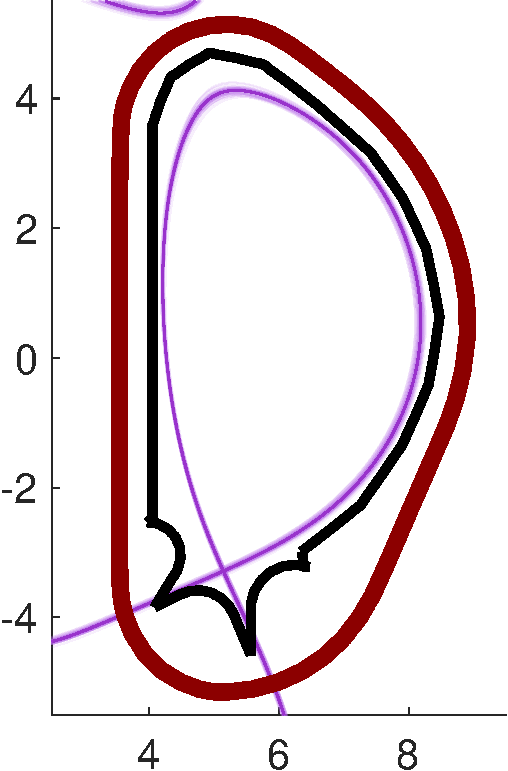
\includegraphics[width=0.19\linewidth]{./figures/QoI_MC_uniform.pdf}
% &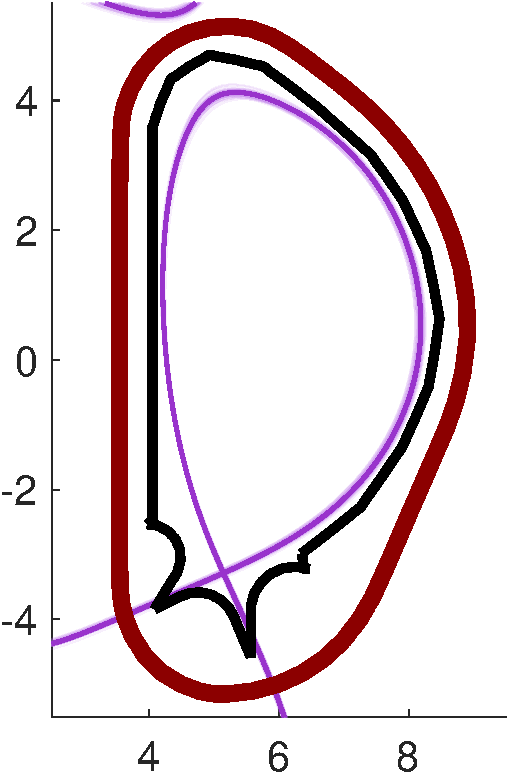
\includegraphics[width=0.19\linewidth]{QoI_MC_surrogate.pdf}
&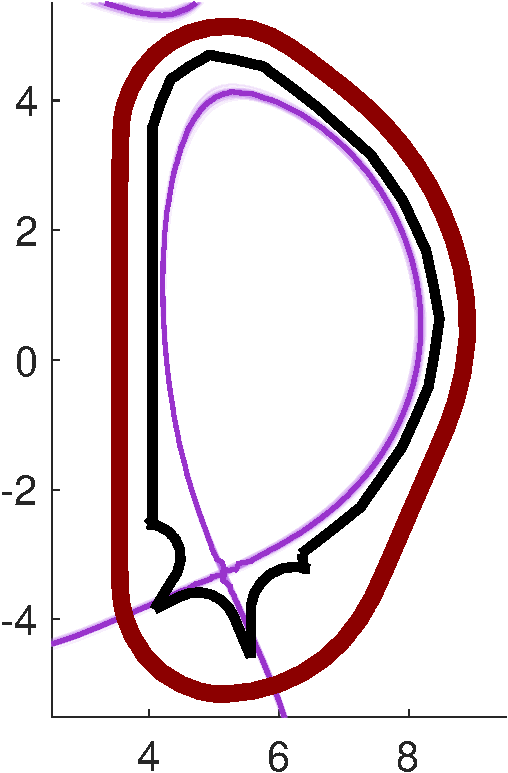
\includegraphics[width=0.19\linewidth]{./figures/QoI_MLMC_uniform_L2norm.pdf} 
% & \includegraphics[width=0.19\linewidth]{QoI_MLMC_surrogate.pdf} 
\\
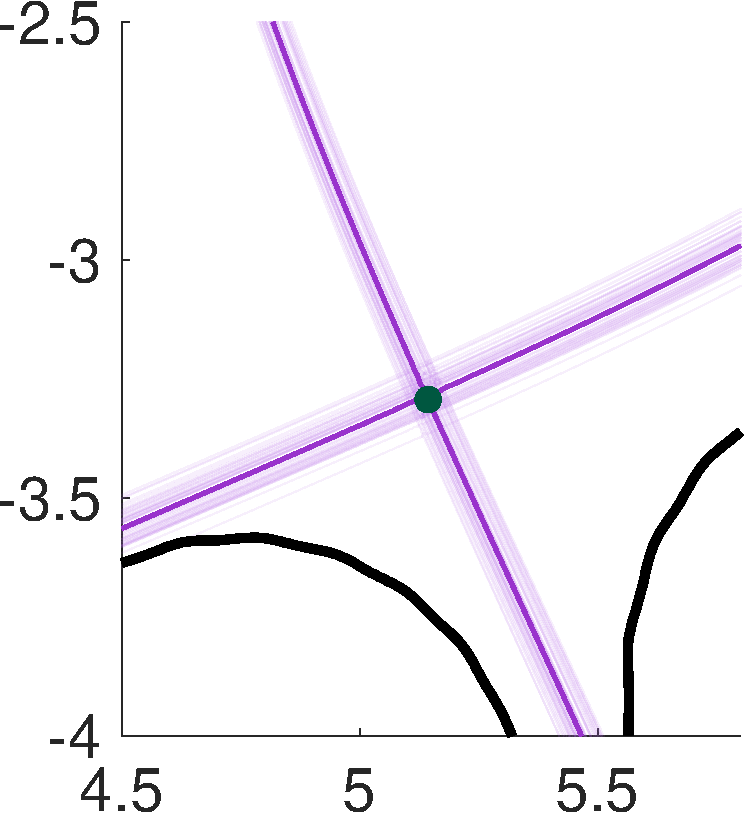
\includegraphics[width=0.19\linewidth]{./figures/QoI_MC_uniform_xptRegion.pdf} 
% &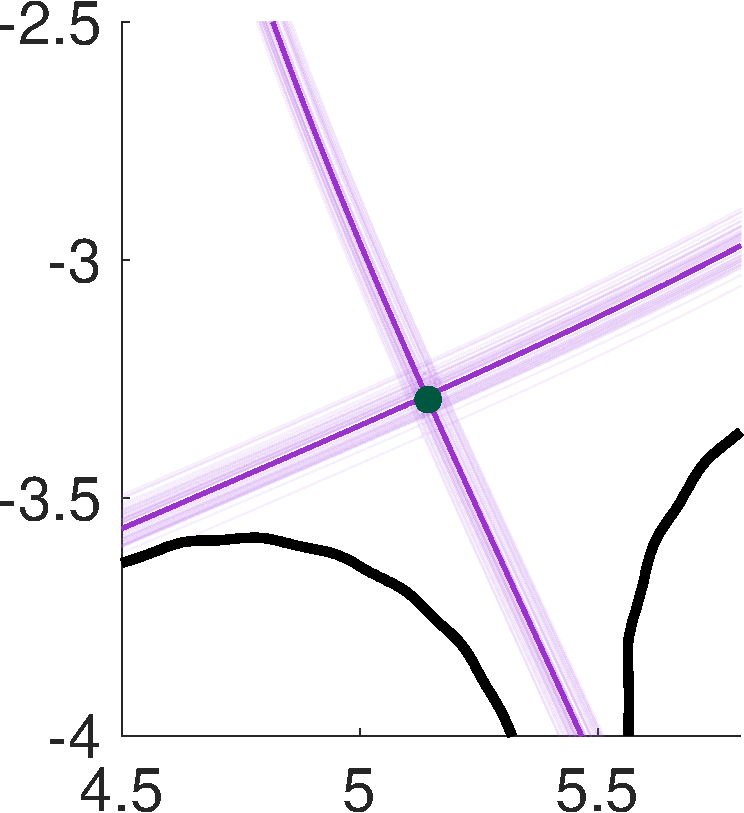
\includegraphics[width=0.19\linewidth]{QoI_MC_surrogate_xptRegion.pdf}
&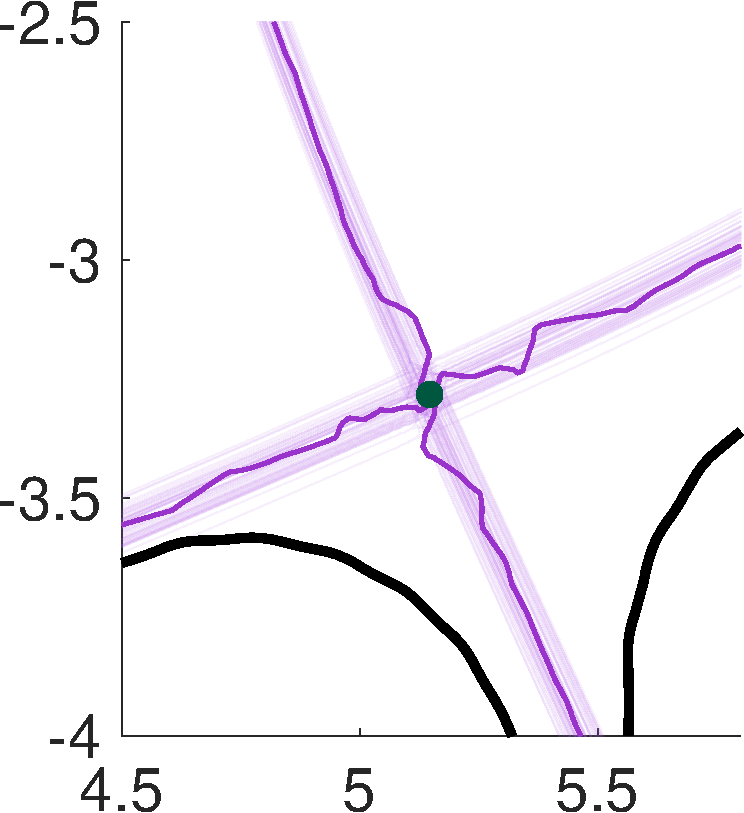
\includegraphics[width=0.19\linewidth]{./figures/QoI_MLMC_uniform_xptRegion_L2norm.pdf} 
% &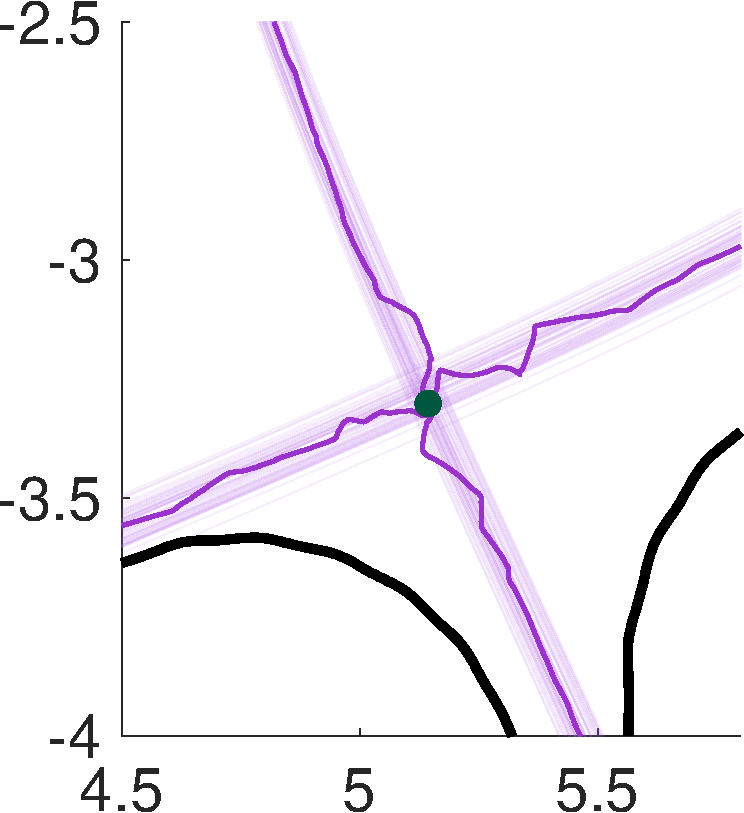
\includegraphics[width=0.19\linewidth]{QoI_MLMC_surrogate_xptRegion.pdf} 
\\[1ex]
\quad MC-FE + Direct Solve &MLMC-FE + Direct Solve &MFMC-FE + Surrogate  \\[-0.5ex]
\end{tabular}
\caption{The overlayed plasma boundaries of 50 random realizations are 
displayed in the top row as violet curves (interpolated to the neighboring 
finer mesh). The solid violet line is the plasma boundary of the expected 
poloidal flux generated with tolerance $\epsilon=4\times 10^{-4}$. 
The inner and outer walls of the reactor are displayed in solid black and 
dark red respectively. The bottom row shows the regions close to the 
x-points in more detail. The dark green dots are the x-points of the expected 
solution. The columns from left to right correspond to simulations using the 
MC-FE approach with the direct solver and surrogate, MLMC-FE with direct 
solver and surrogate. All simulations were performed using the discretization 
level $\ell=5$ on geometry-conforming uniform meshes.} 
\label{fig:QoI_plot}
\end{figure}

\begin{table}[ht]
	\centering
			\scalebox{0.62}{
   \begin{tabular}{c|c|c|c|c|c|c|c|c|c|c|c|c|}
	    \cline{2-7}	
		&\multicolumn{6}{|c|}{ Level $\ell$}\\
			\hline
			\multicolumn{1}{|c|}{$\epsilon$}&0&1&2&3&4&5\\
			\hline
			\multicolumn{1}{|c|}{$8\times 10^{-3} $}&&&5&&&\\
			\multicolumn{1}{|c|}{$6\times 10^{-3} $}&&&7&&&\\
			\multicolumn{1}{|c|}{$4\times 10^{-3} $}&&&&22&&\\
			\multicolumn{1}{|c|}{$2\times 10^{-3} $}&&&&83&&\\
			\multicolumn{1}{|c|}{$10^{-3} $}&&&&&322&\\
			\multicolumn{1}{|c|}{$8\times 10^{-4} $}&&&&&527&\\
			\multicolumn{1}{|c|}{$6\times 10^{-4} $}&&&&&869&\\
                \multicolumn{1}{|c|}{$4\times 10^{-4} $}&&&&&1980&\\
                \multicolumn{1}{|c|}{$2\times 10^{-4} $}&&&&&& 8000$^{\ast}$\!\!\\
			\hline
	\end{tabular}
 \qquad
		\begin{tabular}{c|c|c|c|c|c|c|c|c|c|c|c|c|}
	    \cline{2-7}	
		&\multicolumn{6}{|c|}{ Level $\ell$}\\
			\hline
			\multicolumn{1}{|c|}{$\epsilon$}&0&1&2&3&4&5\\
			\hline
			\multicolumn{1}{|c|}{$8\times 10^{-3} $}&10     &2     &2&&&\\
			\multicolumn{1}{|c|}{$6\times 10^{-3} $}&12     &3     &2&&&\\
			\multicolumn{1}{|c|}{$4\times 10^{-3} $}&32     &5     &2     &2&&\\
			\multicolumn{1}{|c|}{$2\times 10^{-3} $}&152    &26     &4     &2&&\\
			\multicolumn{1}{|c|}{$10^{-3} $}&691   &109    &18     &4     &2&\\
			\multicolumn{1}{|c|}{$8\times 10^{-4} $}&841   &129    &23     &3     &2&\\
			\multicolumn{1}{|c|}{$6\times 10^{-4} $}&1610         &231          &40           &8           &2&\\
                \multicolumn{1}{|c|}{$4\times 10^{-4} $}&3791         &589         &104          &15           &3&\\
                \multicolumn{1}{|c|}{$2\times 10^{-4} $}&15859        &2344         &375          &62          &13           &2\\
			\hline
	\end{tabular}
 \qquad
		\begin{tabular}{c|c|c|c|c|c|c|c|c|c|c|c|c|c|c|c|c|c|}
	    \cline{2-7}	
		&\multicolumn{6}{|c|}{ Level $\ell$}\\
			\hline
			\multicolumn{1}{|c|}{$\epsilon$}&0&1&2&3&4&5\\
			\hline
			\multicolumn{1}{|c|}{$8\times 10^{-3} $}&&&&&&\\
			\multicolumn{1}{|c|}{$6\times 10^{-3} $}&&&&&&\\
			\multicolumn{1}{|c|}{$4\times 10^{-3} $}&&&&&&\\
			\multicolumn{1}{|c|}{$2\times 10^{-3} $}&&&&&&\\
			\multicolumn{1}{|c|}{$10^{-3} $}&&&&&&\\
			\multicolumn{1}{|c|}{$8\times 10^{-4} $}&&&&&&\\
                \multicolumn{1}{|c|}{$6\times 10^{-4} $}&&&&&&\\
			\multicolumn{1}{|c|}{$4\times 10^{-4} $}&&&&&&\\
                \multicolumn{1}{|c|}{$2\times 10^{-4} $}&&&&&&\\
			\hline
	\end{tabular}
 
 }
	\caption{The optimal sample size estimation for MC-FE (left), uniform MLMC-FE (middle), and MFMC-FE (right). The simulations were conducted for a variety of choices of $\epsilon$. The computational cost associated with a tolerance of $\epsilon = 2\times 10^{-4}$ for Monte Carlo was prohibitive; the entry in the table for this tolerance (with an asterisk) is an estimate.}
	\label{Tab:SampleSize}
\end{table}


\section{Acknowledgment}\label{sec:Acknowledgment}

This work was supported in part by AFOSR Grant FA9550-22-1-0004,
by the Big-Data Private-Cloud Research Cyberinfrastructure MRI-award funded by NSF under grant CNS-1338099 
and by Rice University's Center for Research Computing. 

%\bibliographystyle{abbrv}
\bibliographystyle{alphaurl}
\bibliography{references_liang}
\end{document}


